\documentclass[twoside]{book}

% Packages required by doxygen
\usepackage{fixltx2e}
\usepackage{calc}
\usepackage{doxygen}
\usepackage[export]{adjustbox} % also loads graphicx
\usepackage{graphicx}
\usepackage[utf8]{inputenc}
\usepackage{makeidx}
\usepackage{multicol}
\usepackage{multirow}
\PassOptionsToPackage{warn}{textcomp}
\usepackage{textcomp}
\usepackage[nointegrals]{wasysym}
\usepackage[table]{xcolor}

% Font selection
\usepackage[T1]{fontenc}
\usepackage[scaled=.90]{helvet}
\usepackage{courier}
\usepackage{amssymb}
\usepackage{sectsty}
\renewcommand{\familydefault}{\sfdefault}
\allsectionsfont{%
  \fontseries{bc}\selectfont%
  \color{darkgray}%
}
\renewcommand{\DoxyLabelFont}{%
  \fontseries{bc}\selectfont%
  \color{darkgray}%
}
\newcommand{\+}{\discretionary{\mbox{\scriptsize$\hookleftarrow$}}{}{}}

% Page & text layout
\usepackage{geometry}
\geometry{%
  a4paper,%
  top=2.5cm,%
  bottom=2.5cm,%
  left=2.5cm,%
  right=2.5cm%
}
\tolerance=750
\hfuzz=15pt
\hbadness=750
\setlength{\emergencystretch}{15pt}
\setlength{\parindent}{0cm}
\setlength{\parskip}{3ex plus 2ex minus 2ex}
\makeatletter
\renewcommand{\paragraph}{%
  \@startsection{paragraph}{4}{0ex}{-1.0ex}{1.0ex}{%
    \normalfont\normalsize\bfseries\SS@parafont%
  }%
}
\renewcommand{\subparagraph}{%
  \@startsection{subparagraph}{5}{0ex}{-1.0ex}{1.0ex}{%
    \normalfont\normalsize\bfseries\SS@subparafont%
  }%
}
\makeatother

% Headers & footers
\usepackage{fancyhdr}
\pagestyle{fancyplain}
\fancyhead[LE]{\fancyplain{}{\bfseries\thepage}}
\fancyhead[CE]{\fancyplain{}{}}
\fancyhead[RE]{\fancyplain{}{\bfseries\leftmark}}
\fancyhead[LO]{\fancyplain{}{\bfseries\rightmark}}
\fancyhead[CO]{\fancyplain{}{}}
\fancyhead[RO]{\fancyplain{}{\bfseries\thepage}}
\fancyfoot[LE]{\fancyplain{}{}}
\fancyfoot[CE]{\fancyplain{}{}}
\fancyfoot[RE]{\fancyplain{}{\bfseries\scriptsize Generated by Doxygen }}
\fancyfoot[LO]{\fancyplain{}{\bfseries\scriptsize Generated by Doxygen }}
\fancyfoot[CO]{\fancyplain{}{}}
\fancyfoot[RO]{\fancyplain{}{}}
\renewcommand{\footrulewidth}{0.4pt}
\renewcommand{\chaptermark}[1]{%
  \markboth{#1}{}%
}
\renewcommand{\sectionmark}[1]{%
  \markright{\thesection\ #1}%
}

% Indices & bibliography
\usepackage{natbib}
\usepackage[titles]{tocloft}
\setcounter{tocdepth}{3}
\setcounter{secnumdepth}{5}
\makeindex

% Hyperlinks (required, but should be loaded last)
\usepackage{ifpdf}
\ifpdf
  \usepackage[pdftex,pagebackref=true]{hyperref}
\else
  \usepackage[ps2pdf,pagebackref=true]{hyperref}
\fi
\hypersetup{%
  colorlinks=true,%
  linkcolor=blue,%
  citecolor=blue,%
  unicode%
}

% Custom commands
\newcommand{\clearemptydoublepage}{%
  \newpage{\pagestyle{empty}\cleardoublepage}%
}

\usepackage{caption}
\captionsetup{labelsep=space,justification=centering,font={bf},singlelinecheck=off,skip=4pt,position=top}

%===== C O N T E N T S =====

\begin{document}

% Titlepage & ToC
\hypersetup{pageanchor=false,
             bookmarksnumbered=true,
             pdfencoding=unicode
            }
\pagenumbering{alph}
\begin{titlepage}
\vspace*{7cm}
\begin{center}%
{\Large Grass\+Robotics Common }\\
\vspace*{1cm}
{\large Generated by Doxygen 1.8.13}\\
\end{center}
\end{titlepage}
\clearemptydoublepage
\pagenumbering{roman}
\tableofcontents
\clearemptydoublepage
\pagenumbering{arabic}
\hypersetup{pageanchor=true}

%--- Begin generated contents ---
\chapter{R\+E\+A\+D\+ME}
\label{md__home_jose_ros_ws_src_gr_navigation_gr_map_tools_gr_map_utils_README}
\Hypertarget{md__home_jose_ros_ws_src_gr_navigation_gr_map_tools_gr_map_utils_README}
Based on\+: \href{https://github.com/jcmayoral/multi_map_navigation/tree/master/multi_map_server}{\tt https\+://github.\+com/jcmayoral/multi\+\_\+map\+\_\+navigation/tree/master/multi\+\_\+map\+\_\+server} 
\chapter{gr\+\_\+navigation package}
\label{md__home_jose_ros_ws_src_gr_navigation_README}
\Hypertarget{md__home_jose_ros_ws_src_gr_navigation_README}
\subsection*{Overview of the Approach}



\subsection*{Components on Progess}



\subsection*{Map Representations}

A sample of a hybrid map. 

\subsection*{O\+SM Representations}

Open Street Map to Metric map in Polytunnel. 

Navigation over hybrid map (topologic + metric map).  

\subsubsection*{Semantic Map}

Semantic representation. Place Polytunnel.\+Colors\+: Purple (buildings, containers, polytunnel), Blue(workspace), Pink(\+Robot current row) 

\subsection*{Proximity Monitor}

 
\chapter{Hierarchical Index}
\section{Class Hierarchy}
This inheritance list is sorted roughly, but not completely, alphabetically\+:\begin{DoxyCompactList}
\item Base\+Global\+Planner\begin{DoxyCompactList}
\item \contentsline{section}{gr\+\_\+camera\+\_\+base\+\_\+global\+\_\+planner\+:\+:Global\+Planner}{\pageref{classgr__camera__base__global__planner_1_1GlobalPlanner}}{}
\item \contentsline{section}{gr\+\_\+cutting\+\_\+global\+\_\+planner\+:\+:Global\+Planner}{\pageref{classgr__cutting__global__planner_1_1GlobalPlanner}}{}
\end{DoxyCompactList}
\item \contentsline{section}{mongoutils.\+bcolors}{\pageref{classmongoutils_1_1bcolors}}{}
\item \contentsline{section}{gr\+\_\+line\+\_\+trajectory\+\_\+planner\+:\+:G\+R\+Line\+Planner}{\pageref{classgr__line__trajectory__planner_1_1GRLinePlanner}}{}
\item \contentsline{section}{gr\+\_\+map\+\_\+server\+:\+:G\+R\+Map\+Server}{\pageref{classgr__map__server_1_1GRMapServer}}{}
\item \contentsline{section}{gr\+\_\+sbpl\+\_\+trajectory\+\_\+generator\+:\+:G\+R\+S\+B\+P\+L\+Planner}{\pageref{classgr__sbpl__trajectory__generator_1_1GRSBPLPlanner}}{}
\item \contentsline{section}{gr\+\_\+map\+\_\+utils\+:\+:Map\+Converter\+Interface}{\pageref{classgr__map__utils_1_1MapConverterInterface}}{}
\begin{DoxyCompactList}
\item \contentsline{section}{gr\+\_\+map\+\_\+utils\+:\+:Osm2\+Metric\+Map}{\pageref{classgr__map__utils_1_1Osm2MetricMap}}{}
\item \contentsline{section}{gr\+\_\+map\+\_\+utils\+:\+:Osm2\+Topological\+Map}{\pageref{classgr__map__utils_1_1Osm2TopologicalMap}}{}
\item \contentsline{section}{gr\+\_\+map\+\_\+utils\+:\+:Topological2\+Metric\+Map}{\pageref{classgr__map__utils_1_1Topological2MetricMap}}{}
\end{DoxyCompactList}
\item \contentsline{section}{gr\+\_\+map\+\_\+utils\+:\+:Map\+Manager}{\pageref{classgr__map__utils_1_1MapManager}}{}
\item \contentsline{section}{mongodb\+\_\+map\+\_\+utils\+:\+:Mongo\+D\+B\+Map\+Manager}{\pageref{classmongodb__map__utils_1_1MongoDBMapManager}}{}
\item object\begin{DoxyCompactList}
\item \contentsline{section}{mongoutils.\+Mongo\+Manager}{\pageref{classmongoutils_1_1MongoManager}}{}
\item \contentsline{section}{polyfit.\+Action}{\pageref{classpolyfit_1_1Action}}{}
\end{DoxyCompactList}
\item \contentsline{section}{simple\+\_\+row\+\_\+nav.\+Simple\+Row\+Nav\+Controller}{\pageref{classsimple__row__nav_1_1SimpleRowNavController}}{}
\item \contentsline{section}{mbf\+\_\+complex\+\_\+planner.\+Simple\+Topo\+Planner}{\pageref{classmbf__complex__planner_1_1SimpleTopoPlanner}}{}
\item \contentsline{section}{mbf\+\_\+simple\+\_\+planner.\+Simple\+Topo\+Planner}{\pageref{classmbf__simple__planner_1_1SimpleTopoPlanner}}{}
\item \contentsline{section}{simple\+\_\+planner.\+Simple\+Topo\+Planner}{\pageref{classsimple__planner_1_1SimpleTopoPlanner}}{}
\item State\begin{DoxyCompactList}
\item \contentsline{section}{gr\+\_\+topological\+\_\+navigation.\+states.\+manager.\+Manager}{\pageref{classgr__topological__navigation_1_1states_1_1manager_1_1Manager}}{}
\item \contentsline{section}{gr\+\_\+topological\+\_\+navigation.\+states.\+utils.\+Bag\+Recorder}{\pageref{classgr__topological__navigation_1_1states_1_1utils_1_1BagRecorder}}{}
\end{DoxyCompactList}
\item \contentsline{section}{mongodb\+\_\+map\+\_\+utils\+:\+:Tf\+Frame\+Publisher}{\pageref{classmongodb__map__utils_1_1TfFramePublisher}}{}
\item \contentsline{section}{gr\+\_\+map\+\_\+utils\+:\+:Tf\+Frame\+Publisher}{\pageref{classgr__map__utils_1_1TfFramePublisher}}{}
\item \contentsline{section}{tool\+\_\+utils.\+Tool\+Interface}{\pageref{classtool__utils_1_1ToolInterface}}{}
\item Simple\+Action\+State\begin{DoxyCompactList}
\item \contentsline{section}{gr\+\_\+topological\+\_\+navigation.\+states.\+topological\+\_\+planner.\+Topological\+Planner}{\pageref{classgr__topological__navigation_1_1states_1_1topological__planner_1_1TopologicalPlanner}}{}
\end{DoxyCompactList}
\end{DoxyCompactList}

\chapter{Data Structure Index}
\section{Data Structures}
Here are the data structures with brief descriptions\+:\begin{DoxyCompactList}
\item\contentsline{section}{\hyperlink{classpolyfit_1_1Action}{polyfit.\+Action} }{\pageref{classpolyfit_1_1Action}}{}
\item\contentsline{section}{\hyperlink{classgr__topological__navigation_1_1states_1_1utils_1_1BagRecorder}{gr\+\_\+topological\+\_\+navigation.\+states.\+utils.\+Bag\+Recorder} }{\pageref{classgr__topological__navigation_1_1states_1_1utils_1_1BagRecorder}}{}
\item\contentsline{section}{\hyperlink{classmongoutils_1_1bcolors}{mongoutils.\+bcolors} }{\pageref{classmongoutils_1_1bcolors}}{}
\item\contentsline{section}{\hyperlink{classgr__camera__base__global__planner_1_1GlobalPlanner}{gr\+\_\+camera\+\_\+base\+\_\+global\+\_\+planner\+::\+Global\+Planner} }{\pageref{classgr__camera__base__global__planner_1_1GlobalPlanner}}{}
\item\contentsline{section}{\hyperlink{classgr__cutting__global__planner_1_1GlobalPlanner}{gr\+\_\+cutting\+\_\+global\+\_\+planner\+::\+Global\+Planner} }{\pageref{classgr__cutting__global__planner_1_1GlobalPlanner}}{}
\item\contentsline{section}{\hyperlink{classgr__line__trajectory__planner_1_1GRLinePlanner}{gr\+\_\+line\+\_\+trajectory\+\_\+planner\+::\+G\+R\+Line\+Planner} }{\pageref{classgr__line__trajectory__planner_1_1GRLinePlanner}}{}
\item\contentsline{section}{\hyperlink{classgr__map__server_1_1GRMapServer}{gr\+\_\+map\+\_\+server\+::\+G\+R\+Map\+Server} }{\pageref{classgr__map__server_1_1GRMapServer}}{}
\item\contentsline{section}{\hyperlink{classgr__sbpl__trajectory__generator_1_1GRSBPLPlanner}{gr\+\_\+sbpl\+\_\+trajectory\+\_\+generator\+::\+G\+R\+S\+B\+P\+L\+Planner} }{\pageref{classgr__sbpl__trajectory__generator_1_1GRSBPLPlanner}}{}
\item\contentsline{section}{\hyperlink{classgr__topological__navigation_1_1states_1_1manager_1_1Manager}{gr\+\_\+topological\+\_\+navigation.\+states.\+manager.\+Manager} }{\pageref{classgr__topological__navigation_1_1states_1_1manager_1_1Manager}}{}
\item\contentsline{section}{\hyperlink{classgr__map__utils_1_1MapConverterInterface}{gr\+\_\+map\+\_\+utils\+::\+Map\+Converter\+Interface} }{\pageref{classgr__map__utils_1_1MapConverterInterface}}{}
\item\contentsline{section}{\hyperlink{classgr__map__utils_1_1MapManager}{gr\+\_\+map\+\_\+utils\+::\+Map\+Manager} }{\pageref{classgr__map__utils_1_1MapManager}}{}
\item\contentsline{section}{\hyperlink{classmongodb__map__utils_1_1MongoDBMapManager}{mongodb\+\_\+map\+\_\+utils\+::\+Mongo\+D\+B\+Map\+Manager} }{\pageref{classmongodb__map__utils_1_1MongoDBMapManager}}{}
\item\contentsline{section}{\hyperlink{classmongoutils_1_1MongoManager}{mongoutils.\+Mongo\+Manager} }{\pageref{classmongoutils_1_1MongoManager}}{}
\item\contentsline{section}{\hyperlink{classgr__map__utils_1_1Osm2MetricMap}{gr\+\_\+map\+\_\+utils\+::\+Osm2\+Metric\+Map} }{\pageref{classgr__map__utils_1_1Osm2MetricMap}}{}
\item\contentsline{section}{\hyperlink{classgr__map__utils_1_1Osm2TopologicalMap}{gr\+\_\+map\+\_\+utils\+::\+Osm2\+Topological\+Map} }{\pageref{classgr__map__utils_1_1Osm2TopologicalMap}}{}
\item\contentsline{section}{\hyperlink{classsimple__row__nav_1_1SimpleRowNavController}{simple\+\_\+row\+\_\+nav.\+Simple\+Row\+Nav\+Controller} }{\pageref{classsimple__row__nav_1_1SimpleRowNavController}}{}
\item\contentsline{section}{\hyperlink{classmbf__complex__planner_1_1SimpleTopoPlanner}{mbf\+\_\+complex\+\_\+planner.\+Simple\+Topo\+Planner} }{\pageref{classmbf__complex__planner_1_1SimpleTopoPlanner}}{}
\item\contentsline{section}{\hyperlink{classmbf__simple__planner_1_1SimpleTopoPlanner}{mbf\+\_\+simple\+\_\+planner.\+Simple\+Topo\+Planner} }{\pageref{classmbf__simple__planner_1_1SimpleTopoPlanner}}{}
\item\contentsline{section}{\hyperlink{classsimple__planner_1_1SimpleTopoPlanner}{simple\+\_\+planner.\+Simple\+Topo\+Planner} }{\pageref{classsimple__planner_1_1SimpleTopoPlanner}}{}
\item\contentsline{section}{\hyperlink{classmongodb__map__utils_1_1TfFramePublisher}{mongodb\+\_\+map\+\_\+utils\+::\+Tf\+Frame\+Publisher} }{\pageref{classmongodb__map__utils_1_1TfFramePublisher}}{}
\item\contentsline{section}{\hyperlink{classgr__map__utils_1_1TfFramePublisher}{gr\+\_\+map\+\_\+utils\+::\+Tf\+Frame\+Publisher} }{\pageref{classgr__map__utils_1_1TfFramePublisher}}{}
\item\contentsline{section}{\hyperlink{classtool__utils_1_1ToolInterface}{tool\+\_\+utils.\+Tool\+Interface} }{\pageref{classtool__utils_1_1ToolInterface}}{}
\item\contentsline{section}{\hyperlink{classgr__map__utils_1_1Topological2MetricMap}{gr\+\_\+map\+\_\+utils\+::\+Topological2\+Metric\+Map} }{\pageref{classgr__map__utils_1_1Topological2MetricMap}}{}
\item\contentsline{section}{\hyperlink{classgr__topological__navigation_1_1states_1_1topological__planner_1_1TopologicalPlanner}{gr\+\_\+topological\+\_\+navigation.\+states.\+topological\+\_\+planner.\+Topological\+Planner} }{\pageref{classgr__topological__navigation_1_1states_1_1topological__planner_1_1TopologicalPlanner}}{}
\end{DoxyCompactList}

\chapter{Data Structure Documentation}
\hypertarget{classpolyfit_1_1Action}{}\section{polyfit.\+Action Class Reference}
\label{classpolyfit_1_1Action}\index{polyfit.\+Action@{polyfit.\+Action}}


Inheritance diagram for polyfit.\+Action\+:
\nopagebreak
\begin{figure}[H]
\begin{center}
\leavevmode
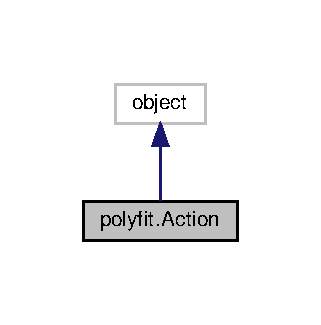
\includegraphics[width=154pt]{classpolyfit_1_1Action__inherit__graph}
\end{center}
\end{figure}


Collaboration diagram for polyfit.\+Action\+:
\nopagebreak
\begin{figure}[H]
\begin{center}
\leavevmode
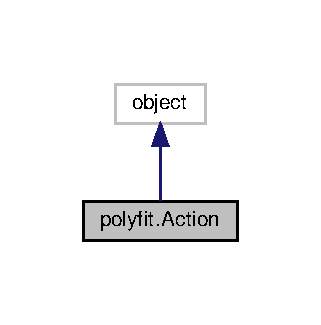
\includegraphics[width=154pt]{classpolyfit_1_1Action__coll__graph}
\end{center}
\end{figure}
\subsection*{Public Member Functions}
\begin{DoxyCompactItemize}
\item 
\mbox{\Hypertarget{classpolyfit_1_1Action_a62f7205a122d0964a7235d438163e1fa}\label{classpolyfit_1_1Action_a62f7205a122d0964a7235d438163e1fa}} 
def {\bfseries \+\_\+\+\_\+init\+\_\+\+\_\+} (self)
\item 
\mbox{\Hypertarget{classpolyfit_1_1Action_a54326e32f816911f53cd1b17d91ae7cb}\label{classpolyfit_1_1Action_a54326e32f816911f53cd1b17d91ae7cb}} 
def {\bfseries myexecution\+\_\+cb} (self, goal)
\item 
\mbox{\Hypertarget{classpolyfit_1_1Action_a15c2a2daa36223bd772bba3934c43958}\label{classpolyfit_1_1Action_a15c2a2daa36223bd772bba3934c43958}} 
def {\bfseries cost2goal} (self, p)
\item 
\mbox{\Hypertarget{classpolyfit_1_1Action_a9281b2dd890c406db377e2cbcfb83aaf}\label{classpolyfit_1_1Action_a9281b2dd890c406db377e2cbcfb83aaf}} 
def {\bfseries complete} (self)
\item 
\mbox{\Hypertarget{classpolyfit_1_1Action_a7614eb119eb9fb6c66e9339e604a3c97}\label{classpolyfit_1_1Action_a7614eb119eb9fb6c66e9339e604a3c97}} 
def {\bfseries set\+Start} (self)
\item 
\mbox{\Hypertarget{classpolyfit_1_1Action_a68dd1ca938aa77500bbe2beb8a97cdc3}\label{classpolyfit_1_1Action_a68dd1ca938aa77500bbe2beb8a97cdc3}} 
def {\bfseries predict} (self, motion, x, y)
\item 
\mbox{\Hypertarget{classpolyfit_1_1Action_a2aa6ed88c720fd2f7ec026f6ce38164b}\label{classpolyfit_1_1Action_a2aa6ed88c720fd2f7ec026f6ce38164b}} 
def {\bfseries apply} (self, motion, states)
\item 
\mbox{\Hypertarget{classpolyfit_1_1Action_a0b2d1187aae443c8863ae5da5f1cce2d}\label{classpolyfit_1_1Action_a0b2d1187aae443c8863ae5da5f1cce2d}} 
def {\bfseries eval\+Motion} (self, x, y, theta)
\item 
\mbox{\Hypertarget{classpolyfit_1_1Action_a30f5d912a21c94bc397d4d44f57fb587}\label{classpolyfit_1_1Action_a30f5d912a21c94bc397d4d44f57fb587}} 
def {\bfseries eval\+Step} (self)
\item 
\mbox{\Hypertarget{classpolyfit_1_1Action_a458e82615d4fe08460047c7357bcf13b}\label{classpolyfit_1_1Action_a458e82615d4fe08460047c7357bcf13b}} 
def {\bfseries plot\+Trajectory} (self)
\item 
\mbox{\Hypertarget{classpolyfit_1_1Action_a07a43fb64e3ab45c5fe62185ca25b41b}\label{classpolyfit_1_1Action_a07a43fb64e3ab45c5fe62185ca25b41b}} 
def {\bfseries run} (self)
\item 
\mbox{\Hypertarget{classpolyfit_1_1Action_a2fcaf278ac12769c5f784171e3e350e1}\label{classpolyfit_1_1Action_a2fcaf278ac12769c5f784171e3e350e1}} 
def {\bfseries draw\+Arrow} (self, A, B)
\item 
\mbox{\Hypertarget{classpolyfit_1_1Action_ac331a10c4e772825ffd69b8d65b04e03}\label{classpolyfit_1_1Action_ac331a10c4e772825ffd69b8d65b04e03}} 
def {\bfseries calculate} (self)
\end{DoxyCompactItemize}
\subsection*{Data Fields}
\begin{DoxyCompactItemize}
\item 
\mbox{\Hypertarget{classpolyfit_1_1Action_af883942b5406961a818b3e8cb5d003a3}\label{classpolyfit_1_1Action_af883942b5406961a818b3e8cb5d003a3}} 
{\bfseries gpath\+\_\+pub}
\item 
\mbox{\Hypertarget{classpolyfit_1_1Action_ae228856c9de4731a75cee2372f5755d8}\label{classpolyfit_1_1Action_ae228856c9de4731a75cee2372f5755d8}} 
{\bfseries lpath\+\_\+pub}
\item 
\mbox{\Hypertarget{classpolyfit_1_1Action_ad6ccdedc655b30dff273f98c55921a50}\label{classpolyfit_1_1Action_ad6ccdedc655b30dff273f98c55921a50}} 
{\bfseries cmd\+\_\+vel}
\item 
\mbox{\Hypertarget{classpolyfit_1_1Action_a3de71a938e62a45661cba27d3bdbf0b5}\label{classpolyfit_1_1Action_a3de71a938e62a45661cba27d3bdbf0b5}} 
{\bfseries dt}
\item 
\mbox{\Hypertarget{classpolyfit_1_1Action_a95b01e575c27f879202b9f4b80969081}\label{classpolyfit_1_1Action_a95b01e575c27f879202b9f4b80969081}} 
{\bfseries x}
\item 
\mbox{\Hypertarget{classpolyfit_1_1Action_a80a93b084897eca2ab017d96c1e69197}\label{classpolyfit_1_1Action_a80a93b084897eca2ab017d96c1e69197}} 
{\bfseries y}
\item 
\mbox{\Hypertarget{classpolyfit_1_1Action_a8b037603ce7be8925731a80689e113b3}\label{classpolyfit_1_1Action_a8b037603ce7be8925731a80689e113b3}} 
{\bfseries thetas}
\item 
\mbox{\Hypertarget{classpolyfit_1_1Action_a386580ea80dfc115793ee11e04c1c93e}\label{classpolyfit_1_1Action_a386580ea80dfc115793ee11e04c1c93e}} 
{\bfseries final}
\item 
\mbox{\Hypertarget{classpolyfit_1_1Action_a62e68737a3200124675ae2e1da0b467d}\label{classpolyfit_1_1Action_a62e68737a3200124675ae2e1da0b467d}} 
{\bfseries nmotion}
\item 
\mbox{\Hypertarget{classpolyfit_1_1Action_a8e34f606068a3e5894794fbcd7da5238}\label{classpolyfit_1_1Action_a8e34f606068a3e5894794fbcd7da5238}} 
{\bfseries ac}
\item 
\mbox{\Hypertarget{classpolyfit_1_1Action_a9c8e8feb4a06685c4ed68c66a606c865}\label{classpolyfit_1_1Action_a9c8e8feb4a06685c4ed68c66a606c865}} 
{\bfseries max\+\_\+vel}
\item 
\mbox{\Hypertarget{classpolyfit_1_1Action_a31a85e33dc4b9f97c787fdfc6ddc0c62}\label{classpolyfit_1_1Action_a31a85e33dc4b9f97c787fdfc6ddc0c62}} 
{\bfseries v}
\item 
\mbox{\Hypertarget{classpolyfit_1_1Action_a6650ff92c0ea1b4a8415a286ee3f82da}\label{classpolyfit_1_1Action_a6650ff92c0ea1b4a8415a286ee3f82da}} 
{\bfseries s}
\item 
\mbox{\Hypertarget{classpolyfit_1_1Action_a3d0f51fc52f5ea8e438508f89ecaa6e2}\label{classpolyfit_1_1Action_a3d0f51fc52f5ea8e438508f89ecaa6e2}} 
{\bfseries max\+\_\+steer}
\item 
\mbox{\Hypertarget{classpolyfit_1_1Action_ada151e541c2bc5fc9595e0e7c917cd39}\label{classpolyfit_1_1Action_ada151e541c2bc5fc9595e0e7c917cd39}} 
{\bfseries trajectory}
\item 
\mbox{\Hypertarget{classpolyfit_1_1Action_adc9cb4072749085ee4bd0eebd1a4c02f}\label{classpolyfit_1_1Action_adc9cb4072749085ee4bd0eebd1a4c02f}} 
{\bfseries motions}
\item 
\mbox{\Hypertarget{classpolyfit_1_1Action_ad58111eb7225e3f64c4b259ac8778dd3}\label{classpolyfit_1_1Action_ad58111eb7225e3f64c4b259ac8778dd3}} 
{\bfseries vels}
\item 
\mbox{\Hypertarget{classpolyfit_1_1Action_ad8095ca3ac8f39cdd95241ab2322910a}\label{classpolyfit_1_1Action_ad8095ca3ac8f39cdd95241ab2322910a}} 
{\bfseries tf}
\item 
\mbox{\Hypertarget{classpolyfit_1_1Action_aca7065e37dc526ded2e710c1ab6c4ddc}\label{classpolyfit_1_1Action_aca7065e37dc526ded2e710c1ab6c4ddc}} 
{\bfseries startx}
\item 
\mbox{\Hypertarget{classpolyfit_1_1Action_a55565fd9083515b8c36e1ec0849cef1f}\label{classpolyfit_1_1Action_a55565fd9083515b8c36e1ec0849cef1f}} 
{\bfseries starty}
\item 
\mbox{\Hypertarget{classpolyfit_1_1Action_a5267446cb70cf144aab5230f6bcba5d5}\label{classpolyfit_1_1Action_a5267446cb70cf144aab5230f6bcba5d5}} 
{\bfseries starttheta}
\item 
\mbox{\Hypertarget{classpolyfit_1_1Action_a06057a6d211f09f1dd9237d14dfa5973}\label{classpolyfit_1_1Action_a06057a6d211f09f1dd9237d14dfa5973}} 
{\bfseries stop}
\item 
\mbox{\Hypertarget{classpolyfit_1_1Action_a5dadb12886965f5fd51318d84720204f}\label{classpolyfit_1_1Action_a5dadb12886965f5fd51318d84720204f}} 
{\bfseries coeff}
\end{DoxyCompactItemize}


\subsection{Detailed Description}


Definition at line 11 of file polyfit.\+py.



The documentation for this class was generated from the following file\+:\begin{DoxyCompactItemize}
\item 
/home/jose/ros\+\_\+ws/src/gr\+\_\+navigation/gr\+\_\+navigation\+\_\+actions/py\+\_\+polyfit/polyfit.\+py\end{DoxyCompactItemize}

\hypertarget{classgr__topological__navigation_1_1states_1_1utils_1_1BagRecorder}{}\section{gr\+\_\+topological\+\_\+navigation.\+states.\+utils.\+Bag\+Recorder Class Reference}
\label{classgr__topological__navigation_1_1states_1_1utils_1_1BagRecorder}\index{gr\+\_\+topological\+\_\+navigation.\+states.\+utils.\+Bag\+Recorder@{gr\+\_\+topological\+\_\+navigation.\+states.\+utils.\+Bag\+Recorder}}


Inheritance diagram for gr\+\_\+topological\+\_\+navigation.\+states.\+utils.\+Bag\+Recorder\+:
\nopagebreak
\begin{figure}[H]
\begin{center}
\leavevmode
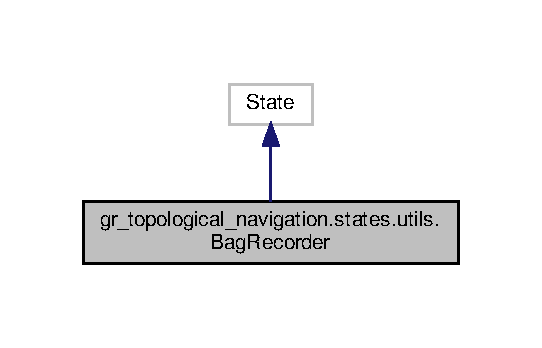
\includegraphics[width=260pt]{classgr__topological__navigation_1_1states_1_1utils_1_1BagRecorder__inherit__graph}
\end{center}
\end{figure}


Collaboration diagram for gr\+\_\+topological\+\_\+navigation.\+states.\+utils.\+Bag\+Recorder\+:
\nopagebreak
\begin{figure}[H]
\begin{center}
\leavevmode
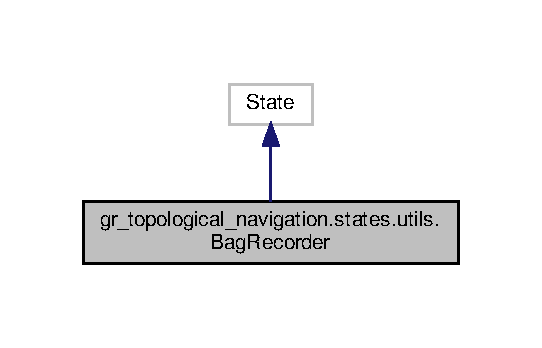
\includegraphics[width=260pt]{classgr__topological__navigation_1_1states_1_1utils_1_1BagRecorder__coll__graph}
\end{center}
\end{figure}
\subsection*{Public Member Functions}
\begin{DoxyCompactItemize}
\item 
\mbox{\Hypertarget{classgr__topological__navigation_1_1states_1_1utils_1_1BagRecorder_ae3cf8fcb5131f95fd4a174222f8f364b}\label{classgr__topological__navigation_1_1states_1_1utils_1_1BagRecorder_ae3cf8fcb5131f95fd4a174222f8f364b}} 
def {\bfseries \+\_\+\+\_\+init\+\_\+\+\_\+} (self, record\+\_\+topics=dict(), desired\+\_\+path=\char`\"{}/home/jose/collection\+\_\+data/topological\+\_\+navigation/\char`\"{}, enable\+\_\+smach=True, start=True)
\item 
\mbox{\Hypertarget{classgr__topological__navigation_1_1states_1_1utils_1_1BagRecorder_a08ecd952e6a51aab3df00daaf7b7711c}\label{classgr__topological__navigation_1_1states_1_1utils_1_1BagRecorder_a08ecd952e6a51aab3df00daaf7b7711c}} 
def {\bfseries start\+Bag} (self)
\item 
\mbox{\Hypertarget{classgr__topological__navigation_1_1states_1_1utils_1_1BagRecorder_a37dc40c02322888061c6ace5f4a0d209}\label{classgr__topological__navigation_1_1states_1_1utils_1_1BagRecorder_a37dc40c02322888061c6ace5f4a0d209}} 
def {\bfseries restart} (self, root\+\_\+name, bag\+\_\+id, close\+\_\+required=True)
\item 
\mbox{\Hypertarget{classgr__topological__navigation_1_1states_1_1utils_1_1BagRecorder_acbde6b6f09f10502cecf9531220a6fee}\label{classgr__topological__navigation_1_1states_1_1utils_1_1BagRecorder_acbde6b6f09f10502cecf9531220a6fee}} 
def {\bfseries execute} (self, userdata)
\item 
\mbox{\Hypertarget{classgr__topological__navigation_1_1states_1_1utils_1_1BagRecorder_ac683946de6e556a59d8f69ab15c94fef}\label{classgr__topological__navigation_1_1states_1_1utils_1_1BagRecorder_ac683946de6e556a59d8f69ab15c94fef}} 
def {\bfseries write\+To\+Bag} (self, topic, msgs)
\item 
\mbox{\Hypertarget{classgr__topological__navigation_1_1states_1_1utils_1_1BagRecorder_ace8e999f3eb6282f3d427473c386e35c}\label{classgr__topological__navigation_1_1states_1_1utils_1_1BagRecorder_ace8e999f3eb6282f3d427473c386e35c}} 
def {\bfseries main\+CB} (self, msg, topic\+\_\+name)
\item 
\mbox{\Hypertarget{classgr__topological__navigation_1_1states_1_1utils_1_1BagRecorder_ac064c83956e44409472ce51a10a32c95}\label{classgr__topological__navigation_1_1states_1_1utils_1_1BagRecorder_ac064c83956e44409472ce51a10a32c95}} 
def {\bfseries close} (self)
\end{DoxyCompactItemize}
\subsection*{Data Fields}
\begin{DoxyCompactItemize}
\item 
\mbox{\Hypertarget{classgr__topological__navigation_1_1states_1_1utils_1_1BagRecorder_aa2595ed3a6dab828fc3773c9fc3e5d88}\label{classgr__topological__navigation_1_1states_1_1utils_1_1BagRecorder_aa2595ed3a6dab828fc3773c9fc3e5d88}} 
{\bfseries is\+\_\+finished}
\item 
\mbox{\Hypertarget{classgr__topological__navigation_1_1states_1_1utils_1_1BagRecorder_ae067a0ac164f2d78fa9014cf183ecd79}\label{classgr__topological__navigation_1_1states_1_1utils_1_1BagRecorder_ae067a0ac164f2d78fa9014cf183ecd79}} 
{\bfseries is\+\_\+bag\+\_\+started}
\item 
\mbox{\Hypertarget{classgr__topological__navigation_1_1states_1_1utils_1_1BagRecorder_ab7edcae916489882d7a79604c65680af}\label{classgr__topological__navigation_1_1states_1_1utils_1_1BagRecorder_ab7edcae916489882d7a79604c65680af}} 
{\bfseries path}
\item 
\mbox{\Hypertarget{classgr__topological__navigation_1_1states_1_1utils_1_1BagRecorder_a9153111d0dfcf5da5cb646718730e996}\label{classgr__topological__navigation_1_1states_1_1utils_1_1BagRecorder_a9153111d0dfcf5da5cb646718730e996}} 
{\bfseries lock}
\item 
\mbox{\Hypertarget{classgr__topological__navigation_1_1states_1_1utils_1_1BagRecorder_a24aab1b485ec6418526495c32f60490a}\label{classgr__topological__navigation_1_1states_1_1utils_1_1BagRecorder_a24aab1b485ec6418526495c32f60490a}} 
{\bfseries bag}
\end{DoxyCompactItemize}


\subsection{Detailed Description}


Definition at line 6 of file utils.\+py.



The documentation for this class was generated from the following file\+:\begin{DoxyCompactItemize}
\item 
/home/jose/ros\+\_\+ws/src/gr\+\_\+navigation/gr\+\_\+navigation\+\_\+managers/gr\+\_\+topological\+\_\+navigation/src/gr\+\_\+topological\+\_\+navigation/states/utils.\+py\end{DoxyCompactItemize}

\hypertarget{classmongoutils_1_1bcolors}{}\section{mongoutils.\+bcolors Class Reference}
\label{classmongoutils_1_1bcolors}\index{mongoutils.\+bcolors@{mongoutils.\+bcolors}}
\subsection*{Static Public Attributes}
\begin{DoxyCompactItemize}
\item 
\mbox{\Hypertarget{classmongoutils_1_1bcolors_acc3d469b1035e2566ef45fe9a52eadc1}\label{classmongoutils_1_1bcolors_acc3d469b1035e2566ef45fe9a52eadc1}} 
string {\bfseries H\+E\+A\+D\+ER} = \textquotesingle{}\textbackslash{}033\mbox{[}95m\textquotesingle{}
\item 
\mbox{\Hypertarget{classmongoutils_1_1bcolors_a2749508660fee0a311a89c4eb27b6ddb}\label{classmongoutils_1_1bcolors_a2749508660fee0a311a89c4eb27b6ddb}} 
string {\bfseries O\+K\+B\+L\+UE} = \textquotesingle{}\textbackslash{}033\mbox{[}94m\textquotesingle{}
\item 
\mbox{\Hypertarget{classmongoutils_1_1bcolors_a24c52c61d75e8be7b7bf32100b3f12af}\label{classmongoutils_1_1bcolors_a24c52c61d75e8be7b7bf32100b3f12af}} 
string {\bfseries O\+K\+C\+Y\+AN} = \textquotesingle{}\textbackslash{}033\mbox{[}96m\textquotesingle{}
\item 
\mbox{\Hypertarget{classmongoutils_1_1bcolors_a02349c7ee9b31866261602ceb3c94c7f}\label{classmongoutils_1_1bcolors_a02349c7ee9b31866261602ceb3c94c7f}} 
string {\bfseries O\+K\+G\+R\+E\+EN} = \textquotesingle{}\textbackslash{}033\mbox{[}92m\textquotesingle{}
\item 
\mbox{\Hypertarget{classmongoutils_1_1bcolors_af8956c2ca03a3953bd7c171f32f8466e}\label{classmongoutils_1_1bcolors_af8956c2ca03a3953bd7c171f32f8466e}} 
string {\bfseries W\+A\+R\+N\+I\+NG} = \textquotesingle{}\textbackslash{}033\mbox{[}93m\textquotesingle{}
\item 
\mbox{\Hypertarget{classmongoutils_1_1bcolors_a9a94bae19b9bd234dfe3ce0cfd29a7d4}\label{classmongoutils_1_1bcolors_a9a94bae19b9bd234dfe3ce0cfd29a7d4}} 
string {\bfseries F\+A\+IL} = \textquotesingle{}\textbackslash{}033\mbox{[}91m\textquotesingle{}
\item 
\mbox{\Hypertarget{classmongoutils_1_1bcolors_abdd175e0ae6545e4bd63b44431b97592}\label{classmongoutils_1_1bcolors_abdd175e0ae6545e4bd63b44431b97592}} 
string {\bfseries E\+N\+DC} = \textquotesingle{}\textbackslash{}033\mbox{[}0m\textquotesingle{}
\item 
\mbox{\Hypertarget{classmongoutils_1_1bcolors_ae508a86d075d5bfc1687d7bc21066a5e}\label{classmongoutils_1_1bcolors_ae508a86d075d5bfc1687d7bc21066a5e}} 
string {\bfseries B\+O\+LD} = \textquotesingle{}\textbackslash{}033\mbox{[}1m\textquotesingle{}
\item 
\mbox{\Hypertarget{classmongoutils_1_1bcolors_afeebb4a9cdd084b9155c27e2c364a3b6}\label{classmongoutils_1_1bcolors_afeebb4a9cdd084b9155c27e2c364a3b6}} 
string {\bfseries U\+N\+D\+E\+R\+L\+I\+NE} = \textquotesingle{}\textbackslash{}033\mbox{[}4m\textquotesingle{}
\end{DoxyCompactItemize}


\subsection{Detailed Description}


Definition at line 5 of file mongoutils.\+py.



The documentation for this class was generated from the following file\+:\begin{DoxyCompactItemize}
\item 
/home/jose/ros\+\_\+ws/src/gr\+\_\+navigation/gr\+\_\+navigation\+\_\+managers/gr\+\_\+simple\+\_\+topological\+\_\+navigation/mongoutils.\+py\end{DoxyCompactItemize}

\hypertarget{classgr__camera__base__global__planner_1_1GlobalPlanner}{}\section{gr\+\_\+camera\+\_\+base\+\_\+global\+\_\+planner\+:\+:Global\+Planner Class Reference}
\label{classgr__camera__base__global__planner_1_1GlobalPlanner}\index{gr\+\_\+camera\+\_\+base\+\_\+global\+\_\+planner\+::\+Global\+Planner@{gr\+\_\+camera\+\_\+base\+\_\+global\+\_\+planner\+::\+Global\+Planner}}


Inheritance diagram for gr\+\_\+camera\+\_\+base\+\_\+global\+\_\+planner\+:\+:Global\+Planner\+:
\nopagebreak
\begin{figure}[H]
\begin{center}
\leavevmode
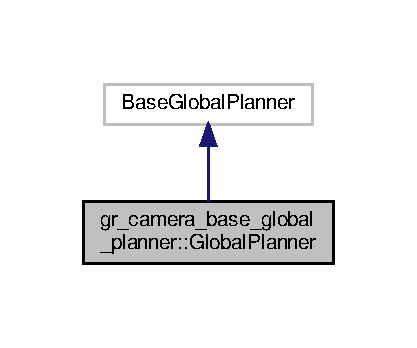
\includegraphics[width=200pt]{classgr__camera__base__global__planner_1_1GlobalPlanner__inherit__graph}
\end{center}
\end{figure}


Collaboration diagram for gr\+\_\+camera\+\_\+base\+\_\+global\+\_\+planner\+:\+:Global\+Planner\+:
\nopagebreak
\begin{figure}[H]
\begin{center}
\leavevmode
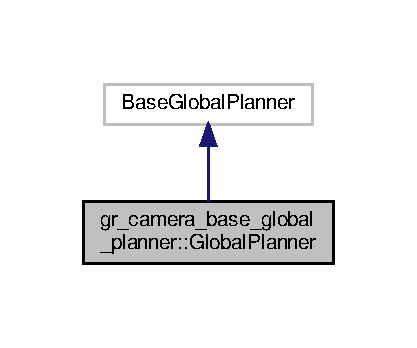
\includegraphics[width=200pt]{classgr__camera__base__global__planner_1_1GlobalPlanner__coll__graph}
\end{center}
\end{figure}
\subsection*{Public Member Functions}
\begin{DoxyCompactItemize}
\item 
\mbox{\Hypertarget{classgr__camera__base__global__planner_1_1GlobalPlanner_af9c3b606d62a2929f7adb00c319bf5ce}\label{classgr__camera__base__global__planner_1_1GlobalPlanner_af9c3b606d62a2929f7adb00c319bf5ce}} 
{\bfseries Global\+Planner} (std\+::string name, costmap\+\_\+2d\+::\+Costmap2\+D\+R\+OS $\ast$costmap\+\_\+ros)
\item 
void \hyperlink{classgr__camera__base__global__planner_1_1GlobalPlanner_a73f1fcbc761007de417426be022642e9}{initialize} (std\+::string name, costmap\+\_\+2d\+::\+Costmap2\+D\+R\+OS $\ast$costmap\+\_\+ros)
\item 
\mbox{\Hypertarget{classgr__camera__base__global__planner_1_1GlobalPlanner_a50a48ecf11b746a10cbd6a76ff4e263f}\label{classgr__camera__base__global__planner_1_1GlobalPlanner_a50a48ecf11b746a10cbd6a76ff4e263f}} 
bool {\bfseries make\+Plan} (const geometry\+\_\+msgs\+::\+Pose\+Stamped \&start, const geometry\+\_\+msgs\+::\+Pose\+Stamped \&goal, std\+::vector$<$ geometry\+\_\+msgs\+::\+Pose\+Stamped $>$ \&plan)
\end{DoxyCompactItemize}


\subsection{Detailed Description}


Definition at line 21 of file global\+\_\+planner.\+h.



\subsection{Member Function Documentation}
\mbox{\Hypertarget{classgr__camera__base__global__planner_1_1GlobalPlanner_a73f1fcbc761007de417426be022642e9}\label{classgr__camera__base__global__planner_1_1GlobalPlanner_a73f1fcbc761007de417426be022642e9}} 
\index{gr\+\_\+camera\+\_\+base\+\_\+global\+\_\+planner\+::\+Global\+Planner@{gr\+\_\+camera\+\_\+base\+\_\+global\+\_\+planner\+::\+Global\+Planner}!initialize@{initialize}}
\index{initialize@{initialize}!gr\+\_\+camera\+\_\+base\+\_\+global\+\_\+planner\+::\+Global\+Planner@{gr\+\_\+camera\+\_\+base\+\_\+global\+\_\+planner\+::\+Global\+Planner}}
\subsubsection{\texorpdfstring{initialize()}{initialize()}}
{\footnotesize\ttfamily void gr\+\_\+camera\+\_\+base\+\_\+global\+\_\+planner\+::\+Global\+Planner\+::initialize (\begin{DoxyParamCaption}\item[{std\+::string}]{name,  }\item[{costmap\+\_\+2d\+::\+Costmap2\+D\+R\+OS $\ast$}]{costmap\+\_\+ros }\end{DoxyParamCaption})}

overridden classes from interface nav\+\_\+core\+::\+Base\+Global\+Planner 

Definition at line 21 of file gr\+\_\+camera\+\_\+base\+\_\+global\+\_\+planner.\+cpp.



The documentation for this class was generated from the following files\+:\begin{DoxyCompactItemize}
\item 
/home/jose/ros\+\_\+ws/src/gr\+\_\+navigation/gr\+\_\+navigation\+\_\+actions/gr\+\_\+camera\+\_\+base\+\_\+global\+\_\+planner/include/gr\+\_\+camera\+\_\+base\+\_\+global\+\_\+planner/global\+\_\+planner.\+h\item 
/home/jose/ros\+\_\+ws/src/gr\+\_\+navigation/gr\+\_\+navigation\+\_\+actions/gr\+\_\+camera\+\_\+base\+\_\+global\+\_\+planner/src/gr\+\_\+camera\+\_\+base\+\_\+global\+\_\+planner.\+cpp\end{DoxyCompactItemize}

\hypertarget{classgr__cutting__global__planner_1_1GlobalPlanner}{}\section{gr\+\_\+cutting\+\_\+global\+\_\+planner\+:\+:Global\+Planner Class Reference}
\label{classgr__cutting__global__planner_1_1GlobalPlanner}\index{gr\+\_\+cutting\+\_\+global\+\_\+planner\+::\+Global\+Planner@{gr\+\_\+cutting\+\_\+global\+\_\+planner\+::\+Global\+Planner}}


Inheritance diagram for gr\+\_\+cutting\+\_\+global\+\_\+planner\+:\+:Global\+Planner\+:
\nopagebreak
\begin{figure}[H]
\begin{center}
\leavevmode
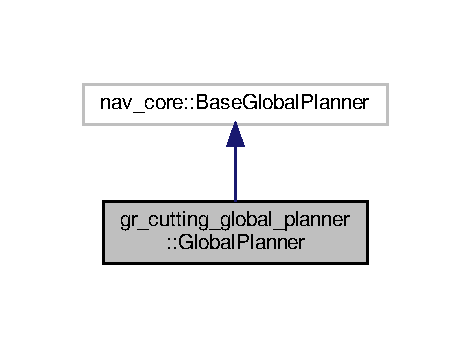
\includegraphics[width=226pt]{classgr__cutting__global__planner_1_1GlobalPlanner__inherit__graph}
\end{center}
\end{figure}


Collaboration diagram for gr\+\_\+cutting\+\_\+global\+\_\+planner\+:\+:Global\+Planner\+:
\nopagebreak
\begin{figure}[H]
\begin{center}
\leavevmode
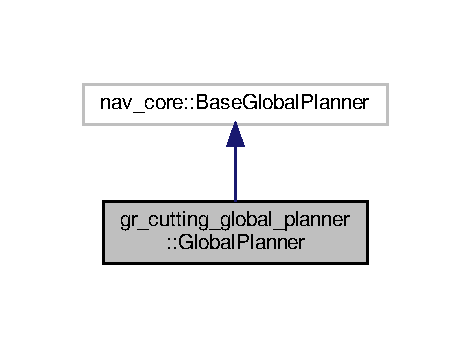
\includegraphics[width=226pt]{classgr__cutting__global__planner_1_1GlobalPlanner__coll__graph}
\end{center}
\end{figure}
\subsection*{Public Member Functions}
\begin{DoxyCompactItemize}
\item 
\mbox{\Hypertarget{classgr__cutting__global__planner_1_1GlobalPlanner_a7a3adcfe1169d597066e4e9c796c1d2b}\label{classgr__cutting__global__planner_1_1GlobalPlanner_a7a3adcfe1169d597066e4e9c796c1d2b}} 
{\bfseries Global\+Planner} (std\+::string name, costmap\+\_\+2d\+::\+Costmap2\+D\+R\+OS $\ast$costmap\+\_\+ros)
\item 
void \hyperlink{classgr__cutting__global__planner_1_1GlobalPlanner_af25c7f31b7b75f49b3a7b2c44cf86c47}{initialize} (std\+::string name, costmap\+\_\+2d\+::\+Costmap2\+D\+R\+OS $\ast$costmap\+\_\+ros)
\item 
\mbox{\Hypertarget{classgr__cutting__global__planner_1_1GlobalPlanner_a919c1fee9e8a8b8adba3b5b2aaf3fd25}\label{classgr__cutting__global__planner_1_1GlobalPlanner_a919c1fee9e8a8b8adba3b5b2aaf3fd25}} 
bool {\bfseries make\+Plan} (const geometry\+\_\+msgs\+::\+Pose\+Stamped \&start, const geometry\+\_\+msgs\+::\+Pose\+Stamped \&goal, std\+::vector$<$ geometry\+\_\+msgs\+::\+Pose\+Stamped $>$ \&plan)
\item 
\mbox{\Hypertarget{classgr__cutting__global__planner_1_1GlobalPlanner_a8cc0d1ce5cfe14da87fec733ae2875a6}\label{classgr__cutting__global__planner_1_1GlobalPlanner_a8cc0d1ce5cfe14da87fec733ae2875a6}} 
void {\bfseries publish\+Plan} (const std\+::vector$<$ geometry\+\_\+msgs\+::\+Pose\+Stamped $>$ \&path, const string frame\+\_\+id)
\end{DoxyCompactItemize}


\subsection{Detailed Description}


Definition at line 21 of file global\+\_\+planner.\+h.



\subsection{Member Function Documentation}
\mbox{\Hypertarget{classgr__cutting__global__planner_1_1GlobalPlanner_af25c7f31b7b75f49b3a7b2c44cf86c47}\label{classgr__cutting__global__planner_1_1GlobalPlanner_af25c7f31b7b75f49b3a7b2c44cf86c47}} 
\index{gr\+\_\+cutting\+\_\+global\+\_\+planner\+::\+Global\+Planner@{gr\+\_\+cutting\+\_\+global\+\_\+planner\+::\+Global\+Planner}!initialize@{initialize}}
\index{initialize@{initialize}!gr\+\_\+cutting\+\_\+global\+\_\+planner\+::\+Global\+Planner@{gr\+\_\+cutting\+\_\+global\+\_\+planner\+::\+Global\+Planner}}
\subsubsection{\texorpdfstring{initialize()}{initialize()}}
{\footnotesize\ttfamily void gr\+\_\+cutting\+\_\+global\+\_\+planner\+::\+Global\+Planner\+::initialize (\begin{DoxyParamCaption}\item[{std\+::string}]{name,  }\item[{costmap\+\_\+2d\+::\+Costmap2\+D\+R\+OS $\ast$}]{costmap\+\_\+ros }\end{DoxyParamCaption})}

overridden classes from interface nav\+\_\+core\+::\+Base\+Global\+Planner 

Definition at line 18 of file gr\+\_\+cutting\+\_\+global\+\_\+planner.\+cpp.



The documentation for this class was generated from the following files\+:\begin{DoxyCompactItemize}
\item 
/home/jose/ros\+\_\+ws/src/gr\+\_\+navigation/gr\+\_\+navigation\+\_\+actions/gr\+\_\+cutting\+\_\+global\+\_\+planner/include/gr\+\_\+cutting\+\_\+global\+\_\+planner/global\+\_\+planner.\+h\item 
/home/jose/ros\+\_\+ws/src/gr\+\_\+navigation/gr\+\_\+navigation\+\_\+actions/gr\+\_\+cutting\+\_\+global\+\_\+planner/src/gr\+\_\+cutting\+\_\+global\+\_\+planner.\+cpp\end{DoxyCompactItemize}

\hypertarget{classgr__line__trajectory__planner_1_1GRLinePlanner}{}\section{gr\+\_\+line\+\_\+trajectory\+\_\+planner\+:\+:G\+R\+Line\+Planner Class Reference}
\label{classgr__line__trajectory__planner_1_1GRLinePlanner}\index{gr\+\_\+line\+\_\+trajectory\+\_\+planner\+::\+G\+R\+Line\+Planner@{gr\+\_\+line\+\_\+trajectory\+\_\+planner\+::\+G\+R\+Line\+Planner}}
\subsection*{Public Member Functions}
\begin{DoxyCompactItemize}
\item 
\mbox{\Hypertarget{classgr__line__trajectory__planner_1_1GRLinePlanner_a88d48d486912cd2111a37cd9ee8e6b41}\label{classgr__line__trajectory__planner_1_1GRLinePlanner_a88d48d486912cd2111a37cd9ee8e6b41}} 
unsigned char {\bfseries cost\+Map\+Cost\+To\+S\+B\+P\+L\+Cost} (unsigned char newcost)
\item 
\mbox{\Hypertarget{classgr__line__trajectory__planner_1_1GRLinePlanner_a3926e3c5d09fc3e305cbb0d0482d6849}\label{classgr__line__trajectory__planner_1_1GRLinePlanner_a3926e3c5d09fc3e305cbb0d0482d6849}} 
bool {\bfseries make\+Plan} (geometry\+\_\+msgs\+::\+Pose\+Stamped start, geometry\+\_\+msgs\+::\+Pose\+Stamped goal)
\item 
\mbox{\Hypertarget{classgr__line__trajectory__planner_1_1GRLinePlanner_a63d08d3230618e2a9ebafbec6adc2902}\label{classgr__line__trajectory__planner_1_1GRLinePlanner_a63d08d3230618e2a9ebafbec6adc2902}} 
void {\bfseries point\+\_\+cb} (const geometry\+\_\+msgs\+::\+Point\+Stamped\+Const\+Ptr msg)
\item 
\mbox{\Hypertarget{classgr__line__trajectory__planner_1_1GRLinePlanner_ae858beef29eabea796e9e04817a73a77}\label{classgr__line__trajectory__planner_1_1GRLinePlanner_ae858beef29eabea796e9e04817a73a77}} 
void {\bfseries execute\+CB} (const move\+\_\+base\+\_\+msgs\+::\+Move\+Base\+Goal\+Const\+Ptr \&goal)
\item 
\mbox{\Hypertarget{classgr__line__trajectory__planner_1_1GRLinePlanner_aca31ac592682f8711bfb1e62d3bdcd6e}\label{classgr__line__trajectory__planner_1_1GRLinePlanner_aca31ac592682f8711bfb1e62d3bdcd6e}} 
bool {\bfseries execute\+Path} ()
\item 
\mbox{\Hypertarget{classgr__line__trajectory__planner_1_1GRLinePlanner_aba069d975df5aef6cb14a287fd9597eb}\label{classgr__line__trajectory__planner_1_1GRLinePlanner_aba069d975df5aef6cb14a287fd9597eb}} 
void {\bfseries odom\+\_\+cb} (const nav\+\_\+msgs\+::\+Odometry\+Const\+Ptr odom\+\_\+msg)
\item 
\mbox{\Hypertarget{classgr__line__trajectory__planner_1_1GRLinePlanner_ab6d45c340d3fbef152526965b7df1694}\label{classgr__line__trajectory__planner_1_1GRLinePlanner_ab6d45c340d3fbef152526965b7df1694}} 
void {\bfseries set\+Start} ()
\item 
\mbox{\Hypertarget{classgr__line__trajectory__planner_1_1GRLinePlanner_a327e4fac6dc19a81b9bb1b89e5523e0f}\label{classgr__line__trajectory__planner_1_1GRLinePlanner_a327e4fac6dc19a81b9bb1b89e5523e0f}} 
void {\bfseries stop} ()
\item 
\mbox{\Hypertarget{classgr__line__trajectory__planner_1_1GRLinePlanner_a681775de390df9533712b2eb5dff2a48}\label{classgr__line__trajectory__planner_1_1GRLinePlanner_a681775de390df9533712b2eb5dff2a48}} 
double {\bfseries get\+Rotation\+In\+Frame} (geometry\+\_\+msgs\+::\+Pose\+Stamped \&pose, std\+::string frame)
\item 
\mbox{\Hypertarget{classgr__line__trajectory__planner_1_1GRLinePlanner_aee6532aefe21ef5cf6bc64d5a8b40f0b}\label{classgr__line__trajectory__planner_1_1GRLinePlanner_aee6532aefe21ef5cf6bc64d5a8b40f0b}} 
double {\bfseries dist2goal} (const geometry\+\_\+msgs\+::\+Pose goal, const geometry\+\_\+msgs\+::\+Pose pose)
\end{DoxyCompactItemize}


\subsection{Detailed Description}


Definition at line 31 of file line\+\_\+trajectory\+\_\+planner.\+h.



The documentation for this class was generated from the following files\+:\begin{DoxyCompactItemize}
\item 
/home/jose/ros\+\_\+ws/src/gr\+\_\+navigation/gr\+\_\+navigation\+\_\+actions/gr\+\_\+line\+\_\+trajectory\+\_\+planner/include/gr\+\_\+line\+\_\+trajectory\+\_\+planner/line\+\_\+trajectory\+\_\+planner.\+h\item 
/home/jose/ros\+\_\+ws/src/gr\+\_\+navigation/gr\+\_\+navigation\+\_\+actions/gr\+\_\+line\+\_\+trajectory\+\_\+planner/src/line\+\_\+trajectory\+\_\+planner.\+cpp\end{DoxyCompactItemize}

\hypertarget{classgr__map__server_1_1GRMapServer}{}\section{gr\+\_\+map\+\_\+server\+:\+:G\+R\+Map\+Server Class Reference}
\label{classgr__map__server_1_1GRMapServer}\index{gr\+\_\+map\+\_\+server\+::\+G\+R\+Map\+Server@{gr\+\_\+map\+\_\+server\+::\+G\+R\+Map\+Server}}
\subsection*{Protected Member Functions}
\begin{DoxyCompactItemize}
\item 
\mbox{\Hypertarget{classgr__map__server_1_1GRMapServer_aaa0f92a0c22acf23acf8185e8b6863a5}\label{classgr__map__server_1_1GRMapServer_aaa0f92a0c22acf23acf8185e8b6863a5}} 
void {\bfseries execute\+\_\+cb} (const G\+R\+Edges\+Action\+Goal \&goal)
\item 
\mbox{\Hypertarget{classgr__map__server_1_1GRMapServer_a5e562d013ad4f53c4fb5442c7df65519}\label{classgr__map__server_1_1GRMapServer_a5e562d013ad4f53c4fb5442c7df65519}} 
void {\bfseries edges\+\_\+cb} (const visualization\+\_\+msgs\+::\+Marker\+::\+Const\+Ptr \&region)
\end{DoxyCompactItemize}


\subsection{Detailed Description}


Definition at line 12 of file gr\+\_\+map\+\_\+server.\+h.



The documentation for this class was generated from the following files\+:\begin{DoxyCompactItemize}
\item 
/home/jose/ros\+\_\+ws/src/gr\+\_\+navigation/gr\+\_\+map\+\_\+tools/gr\+\_\+map\+\_\+server/include/gr\+\_\+map\+\_\+server/gr\+\_\+map\+\_\+server.\+h\item 
/home/jose/ros\+\_\+ws/src/gr\+\_\+navigation/gr\+\_\+map\+\_\+tools/gr\+\_\+map\+\_\+server/src/gr\+\_\+map\+\_\+server.\+cpp\end{DoxyCompactItemize}

\hypertarget{classgr__sbpl__trajectory__generator_1_1GRSBPLPlanner}{}\section{gr\+\_\+sbpl\+\_\+trajectory\+\_\+generator\+:\+:G\+R\+S\+B\+P\+L\+Planner Class Reference}
\label{classgr__sbpl__trajectory__generator_1_1GRSBPLPlanner}\index{gr\+\_\+sbpl\+\_\+trajectory\+\_\+generator\+::\+G\+R\+S\+B\+P\+L\+Planner@{gr\+\_\+sbpl\+\_\+trajectory\+\_\+generator\+::\+G\+R\+S\+B\+P\+L\+Planner}}
\subsection*{Public Member Functions}
\begin{DoxyCompactItemize}
\item 
\mbox{\Hypertarget{classgr__sbpl__trajectory__generator_1_1GRSBPLPlanner_a74c44dce2e6cc0ba2638e69fee037240}\label{classgr__sbpl__trajectory__generator_1_1GRSBPLPlanner_a74c44dce2e6cc0ba2638e69fee037240}} 
unsigned char {\bfseries cost\+Map\+Cost\+To\+S\+B\+P\+L\+Cost} (unsigned char newcost)
\item 
\mbox{\Hypertarget{classgr__sbpl__trajectory__generator_1_1GRSBPLPlanner_a62f3abfb02b63ad5f86c2a01b4804f22}\label{classgr__sbpl__trajectory__generator_1_1GRSBPLPlanner_a62f3abfb02b63ad5f86c2a01b4804f22}} 
bool {\bfseries make\+Plan} (geometry\+\_\+msgs\+::\+Pose\+Stamped start, geometry\+\_\+msgs\+::\+Pose\+Stamped goal)
\item 
\mbox{\Hypertarget{classgr__sbpl__trajectory__generator_1_1GRSBPLPlanner_a62e7982c686bf2b232789399bb71a1ec}\label{classgr__sbpl__trajectory__generator_1_1GRSBPLPlanner_a62e7982c686bf2b232789399bb71a1ec}} 
void {\bfseries point\+\_\+cb} (const geometry\+\_\+msgs\+::\+Point\+Stamped\+Const\+Ptr msg)
\item 
\mbox{\Hypertarget{classgr__sbpl__trajectory__generator_1_1GRSBPLPlanner_a2491c5d67e909546c09fa3c9c5966749}\label{classgr__sbpl__trajectory__generator_1_1GRSBPLPlanner_a2491c5d67e909546c09fa3c9c5966749}} 
void {\bfseries execute\+CB} (const move\+\_\+base\+\_\+msgs\+::\+Move\+Base\+Goal\+Const\+Ptr \&goal)
\item 
\mbox{\Hypertarget{classgr__sbpl__trajectory__generator_1_1GRSBPLPlanner_a736f1960b6dfbeb1e554e590e25a80dc}\label{classgr__sbpl__trajectory__generator_1_1GRSBPLPlanner_a736f1960b6dfbeb1e554e590e25a80dc}} 
bool {\bfseries execute\+Path} ()
\item 
\mbox{\Hypertarget{classgr__sbpl__trajectory__generator_1_1GRSBPLPlanner_ab0c9d8baa6c27ce771d2d8fa630882e1}\label{classgr__sbpl__trajectory__generator_1_1GRSBPLPlanner_ab0c9d8baa6c27ce771d2d8fa630882e1}} 
void {\bfseries odom\+\_\+cb} (const nav\+\_\+msgs\+::\+Odometry\+Const\+Ptr odom\+\_\+msg)
\item 
\mbox{\Hypertarget{classgr__sbpl__trajectory__generator_1_1GRSBPLPlanner_af1167b856f9bb17b2ad2337726f94209}\label{classgr__sbpl__trajectory__generator_1_1GRSBPLPlanner_af1167b856f9bb17b2ad2337726f94209}} 
void {\bfseries set\+Start} ()
\item 
\mbox{\Hypertarget{classgr__sbpl__trajectory__generator_1_1GRSBPLPlanner_adb56bd9cd625ad10c048a82d8898860c}\label{classgr__sbpl__trajectory__generator_1_1GRSBPLPlanner_adb56bd9cd625ad10c048a82d8898860c}} 
void {\bfseries stop} ()
\item 
\mbox{\Hypertarget{classgr__sbpl__trajectory__generator_1_1GRSBPLPlanner_a7956e2577d749607d1babf2b7821ec0e}\label{classgr__sbpl__trajectory__generator_1_1GRSBPLPlanner_a7956e2577d749607d1babf2b7821ec0e}} 
double {\bfseries get\+Rotation\+In\+Frame} (geometry\+\_\+msgs\+::\+Pose\+Stamped \&pose, std\+::string frame)
\item 
\mbox{\Hypertarget{classgr__sbpl__trajectory__generator_1_1GRSBPLPlanner_a8fc1bca78a23e51ecc02fa119582dc7c}\label{classgr__sbpl__trajectory__generator_1_1GRSBPLPlanner_a8fc1bca78a23e51ecc02fa119582dc7c}} 
double {\bfseries distance2\+Goal} (const geometry\+\_\+msgs\+::\+Pose\+Stamped \&pose)
\end{DoxyCompactItemize}


\subsection{Detailed Description}


Definition at line 31 of file spbl\+\_\+planner\+\_\+wrapper.\+h.



The documentation for this class was generated from the following files\+:\begin{DoxyCompactItemize}
\item 
/home/jose/ros\+\_\+ws/src/gr\+\_\+navigation/gr\+\_\+navigation\+\_\+actions/gr\+\_\+sbpl\+\_\+trajectory\+\_\+generator/include/gr\+\_\+sbpl\+\_\+trajectory\+\_\+generator/spbl\+\_\+planner\+\_\+wrapper.\+h\item 
/home/jose/ros\+\_\+ws/src/gr\+\_\+navigation/gr\+\_\+navigation\+\_\+actions/gr\+\_\+sbpl\+\_\+trajectory\+\_\+generator/src/sbpl\+\_\+planner\+\_\+wrapper.\+cpp\end{DoxyCompactItemize}

\hypertarget{classgr__topological__navigation_1_1states_1_1manager_1_1Manager}{}\section{gr\+\_\+topological\+\_\+navigation.\+states.\+manager.\+Manager Class Reference}
\label{classgr__topological__navigation_1_1states_1_1manager_1_1Manager}\index{gr\+\_\+topological\+\_\+navigation.\+states.\+manager.\+Manager@{gr\+\_\+topological\+\_\+navigation.\+states.\+manager.\+Manager}}


Inheritance diagram for gr\+\_\+topological\+\_\+navigation.\+states.\+manager.\+Manager\+:
\nopagebreak
\begin{figure}[H]
\begin{center}
\leavevmode
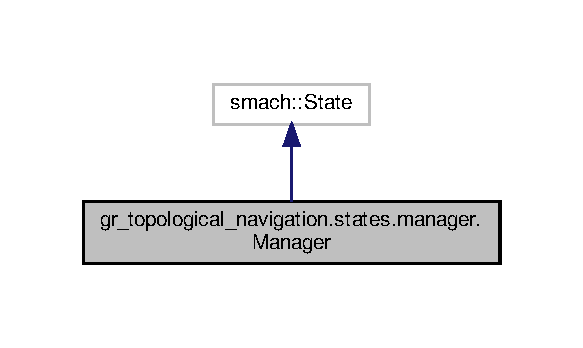
\includegraphics[width=280pt]{classgr__topological__navigation_1_1states_1_1manager_1_1Manager__inherit__graph}
\end{center}
\end{figure}


Collaboration diagram for gr\+\_\+topological\+\_\+navigation.\+states.\+manager.\+Manager\+:
\nopagebreak
\begin{figure}[H]
\begin{center}
\leavevmode
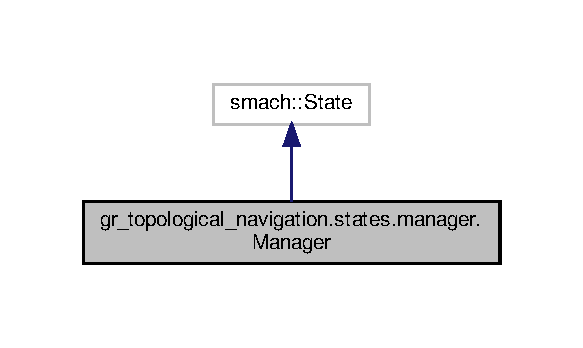
\includegraphics[width=280pt]{classgr__topological__navigation_1_1states_1_1manager_1_1Manager__coll__graph}
\end{center}
\end{figure}
\subsection*{Public Member Functions}
\begin{DoxyCompactItemize}
\item 
\mbox{\Hypertarget{classgr__topological__navigation_1_1states_1_1manager_1_1Manager_a91861f7e96f685bd14a9483b4cdca5d8}\label{classgr__topological__navigation_1_1states_1_1manager_1_1Manager_a91861f7e96f685bd14a9483b4cdca5d8}} 
def {\bfseries \+\_\+\+\_\+init\+\_\+\+\_\+} (self)
\item 
\mbox{\Hypertarget{classgr__topological__navigation_1_1states_1_1manager_1_1Manager_aad8d09e032863827b9a914650097e667}\label{classgr__topological__navigation_1_1states_1_1manager_1_1Manager_aad8d09e032863827b9a914650097e667}} 
def {\bfseries execute} (self, userdata)
\end{DoxyCompactItemize}
\subsection*{Data Fields}
\begin{DoxyCompactItemize}
\item 
\mbox{\Hypertarget{classgr__topological__navigation_1_1states_1_1manager_1_1Manager_ab4672ab015eb022b8c8163743d8ea5a1}\label{classgr__topological__navigation_1_1states_1_1manager_1_1Manager_ab4672ab015eb022b8c8163743d8ea5a1}} 
\hyperlink{classgr__topological__navigation_1_1states_1_1manager_1_1Manager_ab4672ab015eb022b8c8163743d8ea5a1}{rsub}
\begin{DoxyCompactList}\small\item\em H\+A\+CK\+: \end{DoxyCompactList}\end{DoxyCompactItemize}


\subsection{Detailed Description}


Definition at line 5 of file manager.\+py.



The documentation for this class was generated from the following file\+:\begin{DoxyCompactItemize}
\item 
/home/jose/ros\+\_\+ws/src/gr\+\_\+navigation/gr\+\_\+navigation\+\_\+managers/gr\+\_\+topological\+\_\+navigation/src/gr\+\_\+topological\+\_\+navigation/states/manager.\+py\end{DoxyCompactItemize}

\hypertarget{classgr__map__utils_1_1MapConverterInterface}{}\section{gr\+\_\+map\+\_\+utils\+:\+:Map\+Converter\+Interface Class Reference}
\label{classgr__map__utils_1_1MapConverterInterface}\index{gr\+\_\+map\+\_\+utils\+::\+Map\+Converter\+Interface@{gr\+\_\+map\+\_\+utils\+::\+Map\+Converter\+Interface}}


Inheritance diagram for gr\+\_\+map\+\_\+utils\+:\+:Map\+Converter\+Interface\+:
\nopagebreak
\begin{figure}[H]
\begin{center}
\leavevmode
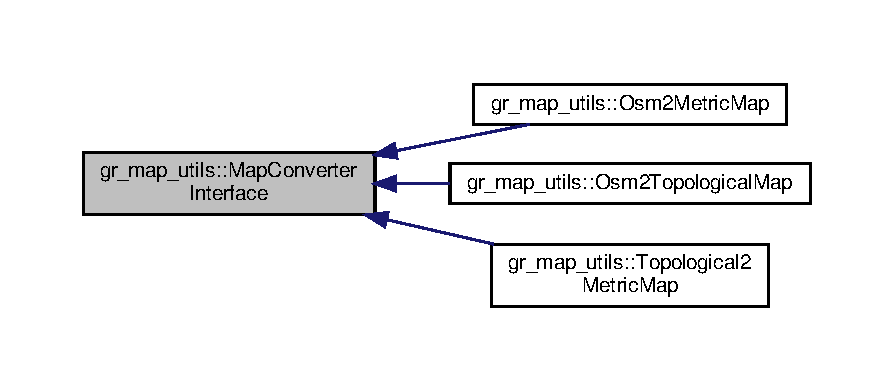
\includegraphics[width=350pt]{classgr__map__utils_1_1MapConverterInterface__inherit__graph}
\end{center}
\end{figure}


Collaboration diagram for gr\+\_\+map\+\_\+utils\+:\+:Map\+Converter\+Interface\+:
\nopagebreak
\begin{figure}[H]
\begin{center}
\leavevmode
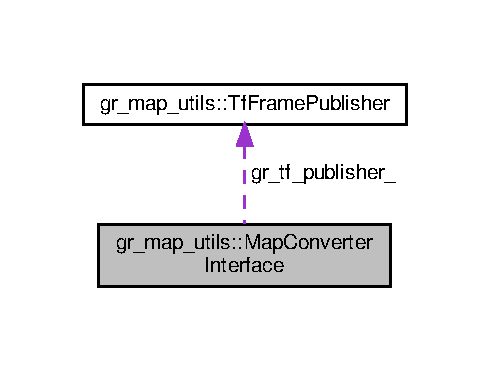
\includegraphics[width=235pt]{classgr__map__utils_1_1MapConverterInterface__coll__graph}
\end{center}
\end{figure}
\subsection*{Public Member Functions}
\begin{DoxyCompactItemize}
\item 
\mbox{\Hypertarget{classgr__map__utils_1_1MapConverterInterface_aff4127c9d962f7aefea06c1c83d56ab3}\label{classgr__map__utils_1_1MapConverterInterface_aff4127c9d962f7aefea06c1c83d56ab3}} 
virtual bool {\bfseries store\+Map} ()=0
\item 
\mbox{\Hypertarget{classgr__map__utils_1_1MapConverterInterface_a817e43868aa64464751a0fe18f93abbd}\label{classgr__map__utils_1_1MapConverterInterface_a817e43868aa64464751a0fe18f93abbd}} 
virtual bool {\bfseries get\+Map\+From\+Topic} ()=0
\item 
\mbox{\Hypertarget{classgr__map__utils_1_1MapConverterInterface_a2977f898bb1d222ebe83a1942309adf9}\label{classgr__map__utils_1_1MapConverterInterface_a2977f898bb1d222ebe83a1942309adf9}} 
virtual bool {\bfseries get\+Map\+From\+Service} ()=0
\item 
\mbox{\Hypertarget{classgr__map__utils_1_1MapConverterInterface_a9f4b08cea1eb98ba3276934dd2607b17}\label{classgr__map__utils_1_1MapConverterInterface_a9f4b08cea1eb98ba3276934dd2607b17}} 
virtual bool {\bfseries get\+Map\+From\+Database} ()=0
\item 
\mbox{\Hypertarget{classgr__map__utils_1_1MapConverterInterface_abd27ecfe34abf1c9af0a8c16741887b2}\label{classgr__map__utils_1_1MapConverterInterface_abd27ecfe34abf1c9af0a8c16741887b2}} 
bool {\bfseries get\+Map} ()
\item 
\mbox{\Hypertarget{classgr__map__utils_1_1MapConverterInterface_a809bff0837d4022d2d6b438436a74a39}\label{classgr__map__utils_1_1MapConverterInterface_a809bff0837d4022d2d6b438436a74a39}} 
virtual void {\bfseries transform\+Map} ()=0
\item 
\mbox{\Hypertarget{classgr__map__utils_1_1MapConverterInterface_ae154736948d178fa0e965c3117952485}\label{classgr__map__utils_1_1MapConverterInterface_ae154736948d178fa0e965c3117952485}} 
virtual void {\bfseries publish\+Maps} ()=0
\end{DoxyCompactItemize}
\subsection*{Protected Attributes}
\begin{DoxyCompactItemize}
\item 
\mbox{\Hypertarget{classgr__map__utils_1_1MapConverterInterface_a7e80da318a096f62e1a0e0866d05eafd}\label{classgr__map__utils_1_1MapConverterInterface_a7e80da318a096f62e1a0e0866d05eafd}} 
mongodb\+\_\+store\+::\+Message\+Store\+Proxy $\ast$ {\bfseries message\+\_\+store\+\_\+}
\item 
\mbox{\Hypertarget{classgr__map__utils_1_1MapConverterInterface_afeaf5a0e9b36d217da89cff6581a396b}\label{classgr__map__utils_1_1MapConverterInterface_afeaf5a0e9b36d217da89cff6581a396b}} 
\hyperlink{classgr__map__utils_1_1TfFramePublisher}{Tf\+Frame\+Publisher} $\ast$ {\bfseries gr\+\_\+tf\+\_\+publisher\+\_\+}
\item 
\mbox{\Hypertarget{classgr__map__utils_1_1MapConverterInterface_ad80118e46635f97762b0c50b5ffbf1ac}\label{classgr__map__utils_1_1MapConverterInterface_ad80118e46635f97762b0c50b5ffbf1ac}} 
bool {\bfseries is\+\_\+map\+\_\+received\+\_\+}
\end{DoxyCompactItemize}


\subsection{Detailed Description}


Definition at line 8 of file map\+\_\+converter\+\_\+interface.\+h.



The documentation for this class was generated from the following file\+:\begin{DoxyCompactItemize}
\item 
/home/jose/ros\+\_\+ws/src/gr\+\_\+navigation/gr\+\_\+map\+\_\+tools/gr\+\_\+map\+\_\+utils/include/gr\+\_\+map\+\_\+utils/map\+\_\+converter\+\_\+interface.\+h\end{DoxyCompactItemize}

\hypertarget{classgr__map__utils_1_1MapManager}{}\section{gr\+\_\+map\+\_\+utils\+:\+:Map\+Manager Class Reference}
\label{classgr__map__utils_1_1MapManager}\index{gr\+\_\+map\+\_\+utils\+::\+Map\+Manager@{gr\+\_\+map\+\_\+utils\+::\+Map\+Manager}}


Collaboration diagram for gr\+\_\+map\+\_\+utils\+:\+:Map\+Manager\+:
\nopagebreak
\begin{figure}[H]
\begin{center}
\leavevmode
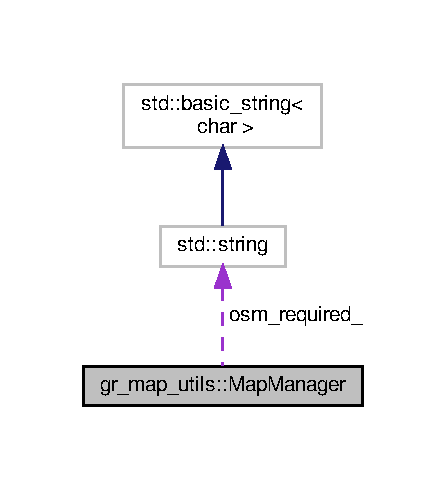
\includegraphics[width=214pt]{classgr__map__utils_1_1MapManager__coll__graph}
\end{center}
\end{figure}
\subsection*{Public Member Functions}
\begin{DoxyCompactItemize}
\item 
\mbox{\Hypertarget{classgr__map__utils_1_1MapManager_af0995b69aceebed7e21dad0a89a8609c}\label{classgr__map__utils_1_1MapManager_af0995b69aceebed7e21dad0a89a8609c}} 
{\bfseries Map\+Manager} (ros\+::\+Node\+Handle nh)
\item 
\mbox{\Hypertarget{classgr__map__utils_1_1MapManager_af094ec9d57f005530b71f5a5d19707ac}\label{classgr__map__utils_1_1MapManager_af094ec9d57f005530b71f5a5d19707ac}} 
bool {\bfseries prepare\+Maps} ()
\item 
\mbox{\Hypertarget{classgr__map__utils_1_1MapManager_a3237c25a17cb93e674ea58daf327b3c2}\label{classgr__map__utils_1_1MapManager_a3237c25a17cb93e674ea58daf327b3c2}} 
void {\bfseries type\+\_\+cb} (const std\+\_\+msgs\+::\+String\+::\+Const\+Ptr type)
\item 
\mbox{\Hypertarget{classgr__map__utils_1_1MapManager_a26ef810a4fde26dc63377bc7f97ec0f4}\label{classgr__map__utils_1_1MapManager_a26ef810a4fde26dc63377bc7f97ec0f4}} 
void {\bfseries check\+\_\+and\+\_\+publish} ()
\end{DoxyCompactItemize}
\subsection*{Protected Attributes}
\begin{DoxyCompactItemize}
\item 
\mbox{\Hypertarget{classgr__map__utils_1_1MapManager_a7fdb5816e1afba98ba2b4caf6d585136}\label{classgr__map__utils_1_1MapManager_a7fdb5816e1afba98ba2b4caf6d585136}} 
std\+::string {\bfseries osm\+\_\+required\+\_\+}
\end{DoxyCompactItemize}


\subsection{Detailed Description}


Definition at line 7 of file map\+\_\+manager.\+hpp.



The documentation for this class was generated from the following file\+:\begin{DoxyCompactItemize}
\item 
/home/jose/ros\+\_\+ws/src/gr\+\_\+navigation/gr\+\_\+map\+\_\+tools/gr\+\_\+map\+\_\+utils/include/gr\+\_\+map\+\_\+utils/map\+\_\+manager.\+hpp\end{DoxyCompactItemize}

\hypertarget{classmongodb__map__utils_1_1MongoDBMapManager}{}\section{mongodb\+\_\+map\+\_\+utils\+:\+:Mongo\+D\+B\+Map\+Manager Class Reference}
\label{classmongodb__map__utils_1_1MongoDBMapManager}\index{mongodb\+\_\+map\+\_\+utils\+::\+Mongo\+D\+B\+Map\+Manager@{mongodb\+\_\+map\+\_\+utils\+::\+Mongo\+D\+B\+Map\+Manager}}
\subsection*{Public Member Functions}
\begin{DoxyCompactItemize}
\item 
\mbox{\Hypertarget{classmongodb__map__utils_1_1MongoDBMapManager_a90ce8194041f68a6f0a1a20e69cc77cb}\label{classmongodb__map__utils_1_1MongoDBMapManager_a90ce8194041f68a6f0a1a20e69cc77cb}} 
void {\bfseries store\+Message} ()
\item 
\mbox{\Hypertarget{classmongodb__map__utils_1_1MongoDBMapManager_a32e14cda48839311bf4bd6c065894c6f}\label{classmongodb__map__utils_1_1MongoDBMapManager_a32e14cda48839311bf4bd6c065894c6f}} 
void {\bfseries get\+Map\+Frame} ()
\item 
\mbox{\Hypertarget{classmongodb__map__utils_1_1MongoDBMapManager_a4cd381d2201f8ffbfddf4804aca15911}\label{classmongodb__map__utils_1_1MongoDBMapManager_a4cd381d2201f8ffbfddf4804aca15911}} 
void {\bfseries publish\+Stuff} ()
\item 
\mbox{\Hypertarget{classmongodb__map__utils_1_1MongoDBMapManager_ae9f4867ef8d48dbc9df9ff28ea5eeb2d}\label{classmongodb__map__utils_1_1MongoDBMapManager_ae9f4867ef8d48dbc9df9ff28ea5eeb2d}} 
bool {\bfseries update\+\_\+frame\+\_\+callback} (std\+\_\+srvs\+::\+Trigger\+::\+Request \&request, std\+\_\+srvs\+::\+Trigger\+::\+Response \&response)
\end{DoxyCompactItemize}


\subsection{Detailed Description}


Definition at line 10 of file mongodb\+\_\+map\+\_\+manager.\+h.



The documentation for this class was generated from the following files\+:\begin{DoxyCompactItemize}
\item 
/home/jose/ros\+\_\+ws/src/gr\+\_\+navigation/gr\+\_\+map\+\_\+tools/mongodb\+\_\+map\+\_\+utils/include/mongodb\+\_\+map\+\_\+utils/mongodb\+\_\+map\+\_\+manager.\+h\item 
/home/jose/ros\+\_\+ws/src/gr\+\_\+navigation/gr\+\_\+map\+\_\+tools/mongodb\+\_\+map\+\_\+utils/src/mongodb\+\_\+map\+\_\+manager.\+cpp\end{DoxyCompactItemize}

\hypertarget{classmongoutils_1_1MongoManager}{}\section{mongoutils.\+Mongo\+Manager Class Reference}
\label{classmongoutils_1_1MongoManager}\index{mongoutils.\+Mongo\+Manager@{mongoutils.\+Mongo\+Manager}}


Inheritance diagram for mongoutils.\+Mongo\+Manager\+:
\nopagebreak
\begin{figure}[H]
\begin{center}
\leavevmode
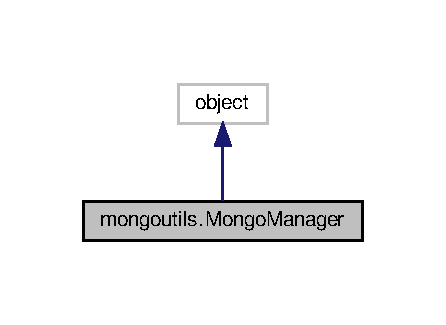
\includegraphics[width=214pt]{classmongoutils_1_1MongoManager__inherit__graph}
\end{center}
\end{figure}


Collaboration diagram for mongoutils.\+Mongo\+Manager\+:
\nopagebreak
\begin{figure}[H]
\begin{center}
\leavevmode
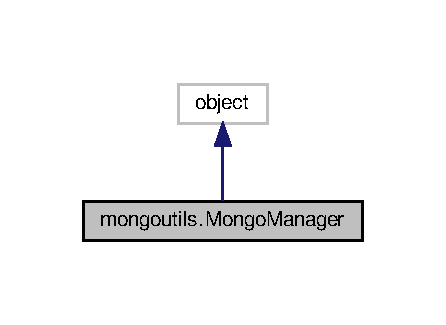
\includegraphics[width=214pt]{classmongoutils_1_1MongoManager__coll__graph}
\end{center}
\end{figure}
\subsection*{Public Member Functions}
\begin{DoxyCompactItemize}
\item 
\mbox{\Hypertarget{classmongoutils_1_1MongoManager_adf09c48a79fcc6fee14357fe0e4e7c48}\label{classmongoutils_1_1MongoManager_adf09c48a79fcc6fee14357fe0e4e7c48}} 
def {\bfseries \+\_\+\+\_\+init\+\_\+\+\_\+} (self, dbname=\char`\"{}execution\+\_\+data\char`\"{})
\item 
\mbox{\Hypertarget{classmongoutils_1_1MongoManager_a14625279a8375d9faa968fb735fe75bd}\label{classmongoutils_1_1MongoManager_a14625279a8375d9faa968fb735fe75bd}} 
def {\bfseries get\+\_\+collection} (self, collname)
\item 
\mbox{\Hypertarget{classmongoutils_1_1MongoManager_ad533c5aa2fe2178adeb7ae79c0b6f9ab}\label{classmongoutils_1_1MongoManager_ad533c5aa2fe2178adeb7ae79c0b6f9ab}} 
def {\bfseries insert\+\_\+in\+\_\+collection} (self, rosmsg, collname)
\item 
\mbox{\Hypertarget{classmongoutils_1_1MongoManager_ae6f80b3ab526c8d216eea64e3cb05de8}\label{classmongoutils_1_1MongoManager_ae6f80b3ab526c8d216eea64e3cb05de8}} 
def {\bfseries query} (self, collname, query=\{\})
\end{DoxyCompactItemize}
\subsection*{Data Fields}
\begin{DoxyCompactItemize}
\item 
\mbox{\Hypertarget{classmongoutils_1_1MongoManager_ae256faf2012042129b91965ace9b36c6}\label{classmongoutils_1_1MongoManager_ae256faf2012042129b91965ace9b36c6}} 
{\bfseries client}
\item 
\mbox{\Hypertarget{classmongoutils_1_1MongoManager_a88927583f24004da9dab59d8e783df54}\label{classmongoutils_1_1MongoManager_a88927583f24004da9dab59d8e783df54}} 
{\bfseries database}
\end{DoxyCompactItemize}


\subsection{Detailed Description}


Definition at line 16 of file mongoutils.\+py.



The documentation for this class was generated from the following file\+:\begin{DoxyCompactItemize}
\item 
/home/jose/ros\+\_\+ws/src/gr\+\_\+navigation/gr\+\_\+navigation\+\_\+managers/gr\+\_\+simple\+\_\+topological\+\_\+navigation/mongoutils.\+py\end{DoxyCompactItemize}

\hypertarget{classgr__map__utils_1_1Osm2MetricMap}{}\section{gr\+\_\+map\+\_\+utils\+:\+:Osm2\+Metric\+Map Class Reference}
\label{classgr__map__utils_1_1Osm2MetricMap}\index{gr\+\_\+map\+\_\+utils\+::\+Osm2\+Metric\+Map@{gr\+\_\+map\+\_\+utils\+::\+Osm2\+Metric\+Map}}


Inheritance diagram for gr\+\_\+map\+\_\+utils\+:\+:Osm2\+Metric\+Map\+:
\nopagebreak
\begin{figure}[H]
\begin{center}
\leavevmode
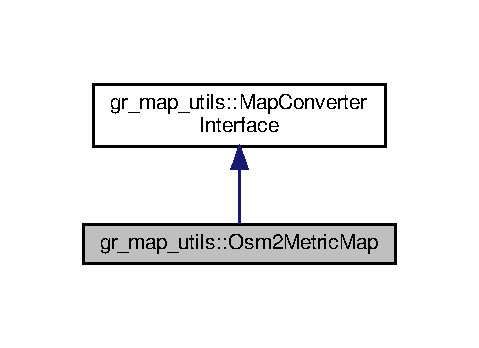
\includegraphics[width=230pt]{classgr__map__utils_1_1Osm2MetricMap__inherit__graph}
\end{center}
\end{figure}


Collaboration diagram for gr\+\_\+map\+\_\+utils\+:\+:Osm2\+Metric\+Map\+:
\nopagebreak
\begin{figure}[H]
\begin{center}
\leavevmode
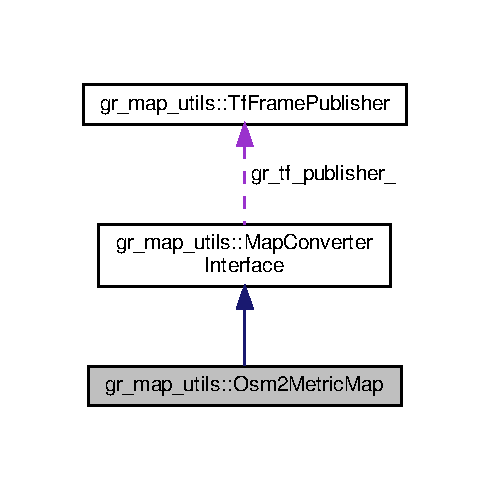
\includegraphics[width=235pt]{classgr__map__utils_1_1Osm2MetricMap__coll__graph}
\end{center}
\end{figure}
\subsection*{Public Member Functions}
\begin{DoxyCompactItemize}
\item 
\mbox{\Hypertarget{classgr__map__utils_1_1Osm2MetricMap_a4391a81c50b65140bb99e5b309b96a22}\label{classgr__map__utils_1_1Osm2MetricMap_a4391a81c50b65140bb99e5b309b96a22}} 
{\bfseries Osm2\+Metric\+Map} (ros\+::\+Node\+Handle nh, std\+::string config\+\_\+file=\char`\"{}config/default\+\_\+osm.\+yaml\char`\"{}, bool init\+\_\+dyn=true)
\item 
\mbox{\Hypertarget{classgr__map__utils_1_1Osm2MetricMap_aaf96863289eacb03fa2a87e285d803d1}\label{classgr__map__utils_1_1Osm2MetricMap_aaf96863289eacb03fa2a87e285d803d1}} 
virtual bool {\bfseries store\+Map} ()
\item 
\mbox{\Hypertarget{classgr__map__utils_1_1Osm2MetricMap_a67377f8e1f6a456d58632b79549a5e58}\label{classgr__map__utils_1_1Osm2MetricMap_a67377f8e1f6a456d58632b79549a5e58}} 
virtual bool {\bfseries get\+Map\+From\+Topic} ()
\item 
\mbox{\Hypertarget{classgr__map__utils_1_1Osm2MetricMap_adeb6cf8a79bbf0ff13efc1f376b1b2bd}\label{classgr__map__utils_1_1Osm2MetricMap_adeb6cf8a79bbf0ff13efc1f376b1b2bd}} 
virtual bool {\bfseries get\+Map\+From\+Service} ()
\item 
\mbox{\Hypertarget{classgr__map__utils_1_1Osm2MetricMap_a594d6074b3760b51be4f7a2d1fafc7fc}\label{classgr__map__utils_1_1Osm2MetricMap_a594d6074b3760b51be4f7a2d1fafc7fc}} 
virtual bool {\bfseries get\+Map\+From\+Database} ()
\item 
\mbox{\Hypertarget{classgr__map__utils_1_1Osm2MetricMap_aa2d77040708a5b215b8bdb89324503ff}\label{classgr__map__utils_1_1Osm2MetricMap_aa2d77040708a5b215b8bdb89324503ff}} 
virtual void {\bfseries transform\+Map} ()
\item 
\mbox{\Hypertarget{classgr__map__utils_1_1Osm2MetricMap_aba7b3d48e16bbdc61756672e807d67ce}\label{classgr__map__utils_1_1Osm2MetricMap_aba7b3d48e16bbdc61756672e807d67ce}} 
virtual void {\bfseries publish\+Maps} ()
\item 
\mbox{\Hypertarget{classgr__map__utils_1_1Osm2MetricMap_a5f117b4a2c6779116ec14d859d40ee61}\label{classgr__map__utils_1_1Osm2MetricMap_a5f117b4a2c6779116ec14d859d40ee61}} 
void {\bfseries publish\+Transform} ()
\item 
\mbox{\Hypertarget{classgr__map__utils_1_1Osm2MetricMap_a2b526463b77e2bdf782c8e19a6f4ce4a}\label{classgr__map__utils_1_1Osm2MetricMap_a2b526463b77e2bdf782c8e19a6f4ce4a}} 
bool {\bfseries add\+O\+S\+M\+Regions} ()
\item 
\mbox{\Hypertarget{classgr__map__utils_1_1Osm2MetricMap_aab4ab1aae454c9ac5b16c831d0027a47}\label{classgr__map__utils_1_1Osm2MetricMap_aab4ab1aae454c9ac5b16c831d0027a47}} 
void {\bfseries osm\+\_\+map\+\_\+cb} (const visualization\+\_\+msgs\+::\+Marker\+Array\+::\+Const\+Ptr \&map)
\item 
\mbox{\Hypertarget{classgr__map__utils_1_1Osm2MetricMap_aea6fd2fc9227cf972d675c20e8564a53}\label{classgr__map__utils_1_1Osm2MetricMap_aea6fd2fc9227cf972d675c20e8564a53}} 
void {\bfseries dyn\+\_\+reconfigure\+CB} (O\+S\+M\+Map\+Converter\+Config \&config, uint32\+\_\+t level)
\item 
\mbox{\Hypertarget{classgr__map__utils_1_1Osm2MetricMap_a0d2437bf5b13131e3bf943a9e582ffbb}\label{classgr__map__utils_1_1Osm2MetricMap_a0d2437bf5b13131e3bf943a9e582ffbb}} 
void {\bfseries fill\+Polygon} (std\+::vector$<$ double $>$x, std\+::vector$<$ double $>$ y)
\item 
\mbox{\Hypertarget{classgr__map__utils_1_1Osm2MetricMap_ad37912f4dcd36142fadfae69ed9fc178}\label{classgr__map__utils_1_1Osm2MetricMap_ad37912f4dcd36142fadfae69ed9fc178}} 
bool {\bfseries map\+Callback} (nav\+\_\+msgs\+::\+Get\+Map\+::\+Request \&req, nav\+\_\+msgs\+::\+Get\+Map\+::\+Response \&res)
\end{DoxyCompactItemize}
\subsection*{Additional Inherited Members}


\subsection{Detailed Description}


Definition at line 32 of file osm\+\_\+to\+\_\+metric\+\_\+converter.\+h.



The documentation for this class was generated from the following files\+:\begin{DoxyCompactItemize}
\item 
/home/jose/ros\+\_\+ws/src/gr\+\_\+navigation/gr\+\_\+map\+\_\+tools/gr\+\_\+map\+\_\+utils/include/gr\+\_\+map\+\_\+utils/osm\+\_\+to\+\_\+metric\+\_\+converter.\+h\item 
/home/jose/ros\+\_\+ws/src/gr\+\_\+navigation/gr\+\_\+map\+\_\+tools/gr\+\_\+map\+\_\+utils/src/osm\+\_\+to\+\_\+metric\+\_\+converter.\+cpp\end{DoxyCompactItemize}

\hypertarget{classgr__map__utils_1_1Osm2TopologicalMap}{}\section{gr\+\_\+map\+\_\+utils\+:\+:Osm2\+Topological\+Map Class Reference}
\label{classgr__map__utils_1_1Osm2TopologicalMap}\index{gr\+\_\+map\+\_\+utils\+::\+Osm2\+Topological\+Map@{gr\+\_\+map\+\_\+utils\+::\+Osm2\+Topological\+Map}}


Inheritance diagram for gr\+\_\+map\+\_\+utils\+:\+:Osm2\+Topological\+Map\+:
\nopagebreak
\begin{figure}[H]
\begin{center}
\leavevmode
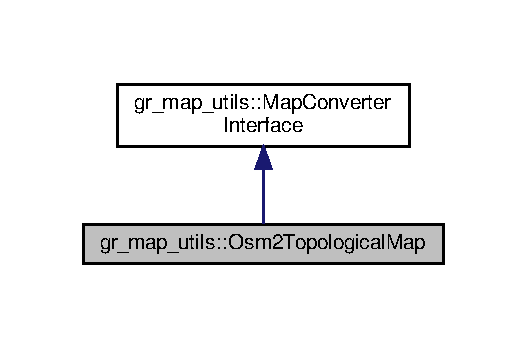
\includegraphics[width=253pt]{classgr__map__utils_1_1Osm2TopologicalMap__inherit__graph}
\end{center}
\end{figure}


Collaboration diagram for gr\+\_\+map\+\_\+utils\+:\+:Osm2\+Topological\+Map\+:
\nopagebreak
\begin{figure}[H]
\begin{center}
\leavevmode
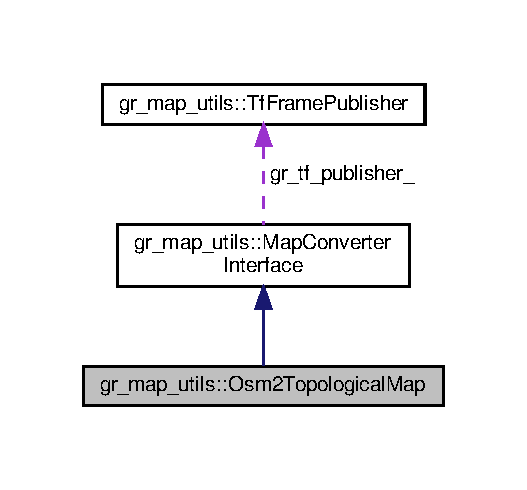
\includegraphics[width=253pt]{classgr__map__utils_1_1Osm2TopologicalMap__coll__graph}
\end{center}
\end{figure}
\subsection*{Public Member Functions}
\begin{DoxyCompactItemize}
\item 
\mbox{\Hypertarget{classgr__map__utils_1_1Osm2TopologicalMap_a4312fea9491b7e04f52f237f165db97d}\label{classgr__map__utils_1_1Osm2TopologicalMap_a4312fea9491b7e04f52f237f165db97d}} 
{\bfseries Osm2\+Topological\+Map} (ros\+::\+Node\+Handle nh)
\item 
\mbox{\Hypertarget{classgr__map__utils_1_1Osm2TopologicalMap_a6cbcd1c5bb8ee339ea159f6a78ba014c}\label{classgr__map__utils_1_1Osm2TopologicalMap_a6cbcd1c5bb8ee339ea159f6a78ba014c}} 
virtual bool {\bfseries store\+Map} ()
\item 
\mbox{\Hypertarget{classgr__map__utils_1_1Osm2TopologicalMap_a252dc6d41ded06a158d4fa77efad3a79}\label{classgr__map__utils_1_1Osm2TopologicalMap_a252dc6d41ded06a158d4fa77efad3a79}} 
virtual bool {\bfseries get\+Map\+From\+Topic} ()
\item 
\mbox{\Hypertarget{classgr__map__utils_1_1Osm2TopologicalMap_a00e019b8428b1408f23dc4fab8f76386}\label{classgr__map__utils_1_1Osm2TopologicalMap_a00e019b8428b1408f23dc4fab8f76386}} 
virtual bool {\bfseries get\+Map\+From\+Service} ()
\item 
\mbox{\Hypertarget{classgr__map__utils_1_1Osm2TopologicalMap_aaadd039386e4e006bc239fa7b443139d}\label{classgr__map__utils_1_1Osm2TopologicalMap_aaadd039386e4e006bc239fa7b443139d}} 
virtual bool {\bfseries get\+Map\+From\+Database} ()
\item 
\mbox{\Hypertarget{classgr__map__utils_1_1Osm2TopologicalMap_a176b71421b4853584522282a271c54c0}\label{classgr__map__utils_1_1Osm2TopologicalMap_a176b71421b4853584522282a271c54c0}} 
virtual void {\bfseries transform\+Map} ()
\item 
\mbox{\Hypertarget{classgr__map__utils_1_1Osm2TopologicalMap_ac8c8cc2a60a3a7ffe3786292da0e1cfb}\label{classgr__map__utils_1_1Osm2TopologicalMap_ac8c8cc2a60a3a7ffe3786292da0e1cfb}} 
virtual void {\bfseries publish\+Maps} ()
\item 
\mbox{\Hypertarget{classgr__map__utils_1_1Osm2TopologicalMap_abb4ae72db1cf25b2f3b2f9cc29d4a5ac}\label{classgr__map__utils_1_1Osm2TopologicalMap_abb4ae72db1cf25b2f3b2f9cc29d4a5ac}} 
void {\bfseries osm\+\_\+map\+\_\+cb} (const visualization\+\_\+msgs\+::\+Marker\+Array\+::\+Const\+Ptr \&map)
\item 
\mbox{\Hypertarget{classgr__map__utils_1_1Osm2TopologicalMap_ab20fa6386acdbf7f6e802a941943eb89}\label{classgr__map__utils_1_1Osm2TopologicalMap_ab20fa6386acdbf7f6e802a941943eb89}} 
void {\bfseries dyn\+\_\+reconfigure\+CB} (O\+S\+M\+Map\+Converter\+Config \&config, uint32\+\_\+t level)
\end{DoxyCompactItemize}
\subsection*{Additional Inherited Members}


\subsection{Detailed Description}


Definition at line 17 of file osm\+\_\+to\+\_\+topological\+\_\+converter.\+h.



The documentation for this class was generated from the following files\+:\begin{DoxyCompactItemize}
\item 
/home/jose/ros\+\_\+ws/src/gr\+\_\+navigation/gr\+\_\+map\+\_\+tools/gr\+\_\+map\+\_\+utils/include/gr\+\_\+map\+\_\+utils/osm\+\_\+to\+\_\+topological\+\_\+converter.\+h\item 
/home/jose/ros\+\_\+ws/src/gr\+\_\+navigation/gr\+\_\+map\+\_\+tools/gr\+\_\+map\+\_\+utils/src/osm\+\_\+to\+\_\+topological\+\_\+converter.\+cpp\end{DoxyCompactItemize}

\hypertarget{classsimple__row__nav_1_1SimpleRowNavController}{}\section{simple\+\_\+row\+\_\+nav.\+Simple\+Row\+Nav\+Controller Class Reference}
\label{classsimple__row__nav_1_1SimpleRowNavController}\index{simple\+\_\+row\+\_\+nav.\+Simple\+Row\+Nav\+Controller@{simple\+\_\+row\+\_\+nav.\+Simple\+Row\+Nav\+Controller}}
\subsection*{Public Member Functions}
\begin{DoxyCompactItemize}
\item 
\mbox{\Hypertarget{classsimple__row__nav_1_1SimpleRowNavController_af7e9d8917110b51d4e02a8227ff47a91}\label{classsimple__row__nav_1_1SimpleRowNavController_af7e9d8917110b51d4e02a8227ff47a91}} 
def {\bfseries \+\_\+\+\_\+init\+\_\+\+\_\+} (self, desired\+\_\+speed=0.\+5, folder=\char`\"{}data\char`\"{}, init\+\_\+bag=True)
\item 
\mbox{\Hypertarget{classsimple__row__nav_1_1SimpleRowNavController_a764796ab31c82680c17b41351dd041c5}\label{classsimple__row__nav_1_1SimpleRowNavController_a764796ab31c82680c17b41351dd041c5}} 
def {\bfseries initialize\+\_\+test} (self)
\item 
\mbox{\Hypertarget{classsimple__row__nav_1_1SimpleRowNavController_a1217a7f9df00251c6b6ea226e29d71fe}\label{classsimple__row__nav_1_1SimpleRowNavController_a1217a7f9df00251c6b6ea226e29d71fe}} 
def {\bfseries voice\+\_\+cb} (self, msg)
\item 
\mbox{\Hypertarget{classsimple__row__nav_1_1SimpleRowNavController_a7f011691d37ba14f39d338583bd7110b}\label{classsimple__row__nav_1_1SimpleRowNavController_a7f011691d37ba14f39d338583bd7110b}} 
def {\bfseries execute\+\_\+cb} (self, goal)
\item 
\mbox{\Hypertarget{classsimple__row__nav_1_1SimpleRowNavController_a97ca81b160bbee9e44c328ec3c89e5fe}\label{classsimple__row__nav_1_1SimpleRowNavController_a97ca81b160bbee9e44c328ec3c89e5fe}} 
def {\bfseries voice\+\_\+cb2} (self, msg)
\item 
\mbox{\Hypertarget{classsimple__row__nav_1_1SimpleRowNavController_a56192e6ab8e7f13b3595e88c1fe3ddf9}\label{classsimple__row__nav_1_1SimpleRowNavController_a56192e6ab8e7f13b3595e88c1fe3ddf9}} 
def {\bfseries swap\+Poses} (self)
\item 
\mbox{\Hypertarget{classsimple__row__nav_1_1SimpleRowNavController_a8dcbbf5c8dd3982882eb3c2e9fbac828}\label{classsimple__row__nav_1_1SimpleRowNavController_a8dcbbf5c8dd3982882eb3c2e9fbac828}} 
def {\bfseries set\+\_\+start\+\_\+pose} (self)
\item 
\mbox{\Hypertarget{classsimple__row__nav_1_1SimpleRowNavController_afc64c528c094ef88fcb8b26547320b53}\label{classsimple__row__nav_1_1SimpleRowNavController_afc64c528c094ef88fcb8b26547320b53}} 
def {\bfseries set\+Poses} (self)
\item 
\mbox{\Hypertarget{classsimple__row__nav_1_1SimpleRowNavController_a2179e3aa0701d8e9de2ce8aaf506e530}\label{classsimple__row__nav_1_1SimpleRowNavController_a2179e3aa0701d8e9de2ce8aaf506e530}} 
def {\bfseries odom\+\_\+cb} (self, msg)
\item 
\mbox{\Hypertarget{classsimple__row__nav_1_1SimpleRowNavController_acca083ef7899f904f8f183b870855a2f}\label{classsimple__row__nav_1_1SimpleRowNavController_acca083ef7899f904f8f183b870855a2f}} 
def {\bfseries is\+\_\+running} (self)
\item 
\mbox{\Hypertarget{classsimple__row__nav_1_1SimpleRowNavController_a038a470844cf5f10dcef99cab0b7e30b}\label{classsimple__row__nav_1_1SimpleRowNavController_a038a470844cf5f10dcef99cab0b7e30b}} 
def {\bfseries check\+\_\+time} (self)
\item 
\mbox{\Hypertarget{classsimple__row__nav_1_1SimpleRowNavController_ab7571969399c685b131ab9321573af8c}\label{classsimple__row__nav_1_1SimpleRowNavController_ab7571969399c685b131ab9321573af8c}} 
def {\bfseries publish} (self, event)
\item 
\mbox{\Hypertarget{classsimple__row__nav_1_1SimpleRowNavController_a05cbeacb3642d80b7ffb56177cd69ffb}\label{classsimple__row__nav_1_1SimpleRowNavController_a05cbeacb3642d80b7ffb56177cd69ffb}} 
def {\bfseries change\+\_\+direction} (self)
\item 
\mbox{\Hypertarget{classsimple__row__nav_1_1SimpleRowNavController_a8af1e4306284bc3c386e9da48fb3908a}\label{classsimple__row__nav_1_1SimpleRowNavController_a8af1e4306284bc3c386e9da48fb3908a}} 
def {\bfseries emergency\+\_\+stop} (self)
\end{DoxyCompactItemize}
\subsection*{Data Fields}
\begin{DoxyCompactItemize}
\item 
\mbox{\Hypertarget{classsimple__row__nav_1_1SimpleRowNavController_abb2539f4a7385dc4823b377a15fe20cc}\label{classsimple__row__nav_1_1SimpleRowNavController_abb2539f4a7385dc4823b377a15fe20cc}} 
{\bfseries twist}
\item 
\mbox{\Hypertarget{classsimple__row__nav_1_1SimpleRowNavController_afef5f72f080bdf0128f2426772398487}\label{classsimple__row__nav_1_1SimpleRowNavController_afef5f72f080bdf0128f2426772398487}} 
{\bfseries desired\+\_\+speed}
\item 
\mbox{\Hypertarget{classsimple__row__nav_1_1SimpleRowNavController_aaa63422a7c78c063446420060ddf68d4}\label{classsimple__row__nav_1_1SimpleRowNavController_aaa63422a7c78c063446420060ddf68d4}} 
{\bfseries is\+\_\+next\+\_\+required}
\item 
\mbox{\Hypertarget{classsimple__row__nav_1_1SimpleRowNavController_afdbd0cb6fe6bf79c7b77686da2bf1a4b}\label{classsimple__row__nav_1_1SimpleRowNavController_afdbd0cb6fe6bf79c7b77686da2bf1a4b}} 
{\bfseries distance}
\item 
\mbox{\Hypertarget{classsimple__row__nav_1_1SimpleRowNavController_afa61fa10a9d899462d6af7905bbb9f4b}\label{classsimple__row__nav_1_1SimpleRowNavController_afa61fa10a9d899462d6af7905bbb9f4b}} 
{\bfseries repetitions}
\item 
\mbox{\Hypertarget{classsimple__row__nav_1_1SimpleRowNavController_a573a9d40e29c9739187e8bc627e77cce}\label{classsimple__row__nav_1_1SimpleRowNavController_a573a9d40e29c9739187e8bc627e77cce}} 
{\bfseries listener}
\item 
\mbox{\Hypertarget{classsimple__row__nav_1_1SimpleRowNavController_adb77f91108152f7addada1b06f477b54}\label{classsimple__row__nav_1_1SimpleRowNavController_adb77f91108152f7addada1b06f477b54}} 
{\bfseries init\+\_\+bag}
\item 
\mbox{\Hypertarget{classsimple__row__nav_1_1SimpleRowNavController_ac52a085c943bd57da0d0d9a7b1851287}\label{classsimple__row__nav_1_1SimpleRowNavController_ac52a085c943bd57da0d0d9a7b1851287}} 
{\bfseries max\+\_\+execution\+\_\+time}
\item 
\mbox{\Hypertarget{classsimple__row__nav_1_1SimpleRowNavController_aa717f2dda9cac22809ca92a6846ead99}\label{classsimple__row__nav_1_1SimpleRowNavController_aa717f2dda9cac22809ca92a6846ead99}} 
{\bfseries start\+\_\+time}
\item 
\mbox{\Hypertarget{classsimple__row__nav_1_1SimpleRowNavController_ac343933aa55836e54cf82f0cb3311716}\label{classsimple__row__nav_1_1SimpleRowNavController_ac343933aa55836e54cf82f0cb3311716}} 
{\bfseries is\+\_\+not\+\_\+aborted}
\item 
\mbox{\Hypertarget{classsimple__row__nav_1_1SimpleRowNavController_af6589d5d5a04758fe5c2181855440cb6}\label{classsimple__row__nav_1_1SimpleRowNavController_af6589d5d5a04758fe5c2181855440cb6}} 
{\bfseries rb}
\item 
\mbox{\Hypertarget{classsimple__row__nav_1_1SimpleRowNavController_af9963e8d921d263e4d64920373ce7ae0}\label{classsimple__row__nav_1_1SimpleRowNavController_af9963e8d921d263e4d64920373ce7ae0}} 
{\bfseries pub}
\item 
\mbox{\Hypertarget{classsimple__row__nav_1_1SimpleRowNavController_a6af0cb851981e6f2010a2159c4c47224}\label{classsimple__row__nav_1_1SimpleRowNavController_a6af0cb851981e6f2010a2159c4c47224}} 
{\bfseries action\+\_\+trigger}
\item 
\mbox{\Hypertarget{classsimple__row__nav_1_1SimpleRowNavController_af56852c83666544e3fe8e3071bfbb38f}\label{classsimple__row__nav_1_1SimpleRowNavController_af56852c83666544e3fe8e3071bfbb38f}} 
{\bfseries ac\+\_\+fb}
\item 
\mbox{\Hypertarget{classsimple__row__nav_1_1SimpleRowNavController_ad385a34fefbb417ae354148063852fec}\label{classsimple__row__nav_1_1SimpleRowNavController_ad385a34fefbb417ae354148063852fec}} 
{\bfseries ac\+\_\+result}
\item 
\mbox{\Hypertarget{classsimple__row__nav_1_1SimpleRowNavController_af97ee0e2a6e358ec9f8aa8434c548cd6}\label{classsimple__row__nav_1_1SimpleRowNavController_af97ee0e2a6e358ec9f8aa8434c548cd6}} 
{\bfseries current\+\_\+motions}
\item 
\mbox{\Hypertarget{classsimple__row__nav_1_1SimpleRowNavController_ace6cdeaa1049fbffa02de4e80b5f7c22}\label{classsimple__row__nav_1_1SimpleRowNavController_ace6cdeaa1049fbffa02de4e80b5f7c22}} 
{\bfseries startpose}
\item 
\mbox{\Hypertarget{classsimple__row__nav_1_1SimpleRowNavController_a8151e1ec16bb80db78301272441f0153}\label{classsimple__row__nav_1_1SimpleRowNavController_a8151e1ec16bb80db78301272441f0153}} 
{\bfseries endpose}
\item 
\mbox{\Hypertarget{classsimple__row__nav_1_1SimpleRowNavController_a7cd3ca7b30d80246c7b73044e95a9020}\label{classsimple__row__nav_1_1SimpleRowNavController_a7cd3ca7b30d80246c7b73044e95a9020}} 
{\bfseries currentpose}
\item 
\mbox{\Hypertarget{classsimple__row__nav_1_1SimpleRowNavController_a5b56e122ebacdc469279ceb15fe9025c}\label{classsimple__row__nav_1_1SimpleRowNavController_a5b56e122ebacdc469279ceb15fe9025c}} 
{\bfseries start}
\item 
\mbox{\Hypertarget{classsimple__row__nav_1_1SimpleRowNavController_aba83feb339258e0091f3e82bcaadd663}\label{classsimple__row__nav_1_1SimpleRowNavController_aba83feb339258e0091f3e82bcaadd663}} 
{\bfseries forward}
\item 
\mbox{\Hypertarget{classsimple__row__nav_1_1SimpleRowNavController_afd8413d9247aedf3e1425ef703ab91b5}\label{classsimple__row__nav_1_1SimpleRowNavController_afd8413d9247aedf3e1425ef703ab91b5}} 
{\bfseries command}
\item 
\mbox{\Hypertarget{classsimple__row__nav_1_1SimpleRowNavController_a9abba4807d494c063ed9017a7fe5a83f}\label{classsimple__row__nav_1_1SimpleRowNavController_a9abba4807d494c063ed9017a7fe5a83f}} 
{\bfseries init\+Pose}
\item 
\mbox{\Hypertarget{classsimple__row__nav_1_1SimpleRowNavController_a9173e0f8b8fd4eaf8f2f878f3dc2d286}\label{classsimple__row__nav_1_1SimpleRowNavController_a9173e0f8b8fd4eaf8f2f878f3dc2d286}} 
{\bfseries pend\+Pose}
\end{DoxyCompactItemize}


\subsection{Detailed Description}


Definition at line 30 of file simple\+\_\+row\+\_\+nav.\+py.



The documentation for this class was generated from the following file\+:\begin{DoxyCompactItemize}
\item 
/home/jose/ros\+\_\+ws/src/gr\+\_\+navigation/gr\+\_\+navigation\+\_\+actions/simple\+\_\+row\+\_\+nav/simple\+\_\+row\+\_\+nav.\+py\end{DoxyCompactItemize}

\hypertarget{classmbf__complex__planner_1_1SimpleTopoPlanner}{}\section{mbf\+\_\+complex\+\_\+planner.\+Simple\+Topo\+Planner Class Reference}
\label{classmbf__complex__planner_1_1SimpleTopoPlanner}\index{mbf\+\_\+complex\+\_\+planner.\+Simple\+Topo\+Planner@{mbf\+\_\+complex\+\_\+planner.\+Simple\+Topo\+Planner}}
\subsection*{Public Member Functions}
\begin{DoxyCompactItemize}
\item 
\mbox{\Hypertarget{classmbf__complex__planner_1_1SimpleTopoPlanner_a72330ca8f10eeeb446663623aa930e12}\label{classmbf__complex__planner_1_1SimpleTopoPlanner_a72330ca8f10eeeb446663623aa930e12}} 
def {\bfseries \+\_\+\+\_\+init\+\_\+\+\_\+} (self)
\item 
\mbox{\Hypertarget{classmbf__complex__planner_1_1SimpleTopoPlanner_aff8d779274db6db0f2b3d5eb49952638}\label{classmbf__complex__planner_1_1SimpleTopoPlanner_aff8d779274db6db0f2b3d5eb49952638}} 
def {\bfseries container\+\_\+cb} (self, is\+\_\+full)
\item 
\mbox{\Hypertarget{classmbf__complex__planner_1_1SimpleTopoPlanner_adb0633463b52460555688439eeb13f3b}\label{classmbf__complex__planner_1_1SimpleTopoPlanner_adb0633463b52460555688439eeb13f3b}} 
def {\bfseries load\+\_\+movebase\+\_\+params} (self)
\item 
\mbox{\Hypertarget{classmbf__complex__planner_1_1SimpleTopoPlanner_a64668d39e5f4ee3502473920e5e7e62e}\label{classmbf__complex__planner_1_1SimpleTopoPlanner_a64668d39e5f4ee3502473920e5e7e62e}} 
def {\bfseries config\+\_\+callback} (self, config)
\item 
\mbox{\Hypertarget{classmbf__complex__planner_1_1SimpleTopoPlanner_a81b512c2eaefa41a43b809b6a361f8a0}\label{classmbf__complex__planner_1_1SimpleTopoPlanner_a81b512c2eaefa41a43b809b6a361f8a0}} 
def {\bfseries move\+\_\+base\+\_\+server} (self, commands, nav\+\_\+mode)
\item 
\mbox{\Hypertarget{classmbf__complex__planner_1_1SimpleTopoPlanner_ab8d7a141999fa9f49490dec83eb543e2}\label{classmbf__complex__planner_1_1SimpleTopoPlanner_ab8d7a141999fa9f49490dec83eb543e2}} 
def {\bfseries active\+\_\+cb} (self)
\item 
\mbox{\Hypertarget{classmbf__complex__planner_1_1SimpleTopoPlanner_a7b52214fb5bd624ac1969ac3320bc881}\label{classmbf__complex__planner_1_1SimpleTopoPlanner_a7b52214fb5bd624ac1969ac3320bc881}} 
def {\bfseries calc\+\_\+distance} (self, a, b)
\item 
\mbox{\Hypertarget{classmbf__complex__planner_1_1SimpleTopoPlanner_ac528fd86c83c3ff614fb163063892a68}\label{classmbf__complex__planner_1_1SimpleTopoPlanner_ac528fd86c83c3ff614fb163063892a68}} 
def {\bfseries feedback\+\_\+cb} (self, feedback)
\item 
\mbox{\Hypertarget{classmbf__complex__planner_1_1SimpleTopoPlanner_ac098aad2b06aca0367df128a046c4749}\label{classmbf__complex__planner_1_1SimpleTopoPlanner_ac098aad2b06aca0367df128a046c4749}} 
def {\bfseries done\+\_\+cb} (self, state, result)
\item 
\mbox{\Hypertarget{classmbf__complex__planner_1_1SimpleTopoPlanner_a830f8e104b9d21ef08fddec3e0ffb635}\label{classmbf__complex__planner_1_1SimpleTopoPlanner_a830f8e104b9d21ef08fddec3e0ffb635}} 
def {\bfseries execute\+\_\+cb} (self, goal)
\item 
\mbox{\Hypertarget{classmbf__complex__planner_1_1SimpleTopoPlanner_a9060d160e1b58128e55f56b426fca37e}\label{classmbf__complex__planner_1_1SimpleTopoPlanner_a9060d160e1b58128e55f56b426fca37e}} 
def {\bfseries map\+\_\+cb} (self, map)
\item 
\mbox{\Hypertarget{classmbf__complex__planner_1_1SimpleTopoPlanner_ac2cb0f8887ca015c4bdfb39f538b78b1}\label{classmbf__complex__planner_1_1SimpleTopoPlanner_ac2cb0f8887ca015c4bdfb39f538b78b1}} 
def {\bfseries wait\+Move\+Base} (self, flag=True)
\item 
\mbox{\Hypertarget{classmbf__complex__planner_1_1SimpleTopoPlanner_a8e3dd4534af258f95b1cf8232ac0135e}\label{classmbf__complex__planner_1_1SimpleTopoPlanner_a8e3dd4534af258f95b1cf8232ac0135e}} 
def {\bfseries go\+\_\+to\+\_\+unload\+\_\+zone} (self, current\+\_\+goal)
\item 
\mbox{\Hypertarget{classmbf__complex__planner_1_1SimpleTopoPlanner_a73461a86ea294480241664a802b48ff3}\label{classmbf__complex__planner_1_1SimpleTopoPlanner_a73461a86ea294480241664a802b48ff3}} 
def {\bfseries wait\+\_\+for\+\_\+unload} (self)
\item 
\mbox{\Hypertarget{classmbf__complex__planner_1_1SimpleTopoPlanner_a9ea75e47ff25f6d96a2e4da1accf009b}\label{classmbf__complex__planner_1_1SimpleTopoPlanner_a9ea75e47ff25f6d96a2e4da1accf009b}} 
def {\bfseries unload\+\_\+cb} (self, msg)
\item 
\mbox{\Hypertarget{classmbf__complex__planner_1_1SimpleTopoPlanner_a9e85fecf600ccd37145bf84492211ce2}\label{classmbf__complex__planner_1_1SimpleTopoPlanner_a9e85fecf600ccd37145bf84492211ce2}} 
def {\bfseries perform\+\_\+motion} (self, goal, id, constrain\+\_\+motion, mode)
\item 
def \hyperlink{classmbf__complex__planner_1_1SimpleTopoPlanner_a9eb51a878e3f7891274bad1e253b61f4}{execute\+\_\+plan} (self, mode, span=0)
\item 
\mbox{\Hypertarget{classmbf__complex__planner_1_1SimpleTopoPlanner_a595c1c401ab85c83fd0a4506b1b44765}\label{classmbf__complex__planner_1_1SimpleTopoPlanner_a595c1c401ab85c83fd0a4506b1b44765}} 
def {\bfseries get\+\_\+topological\+\_\+plan} (self, startnode, goalnode)
\item 
\mbox{\Hypertarget{classmbf__complex__planner_1_1SimpleTopoPlanner_a085cd3dd1cf3ef6e4e712b37baa67019}\label{classmbf__complex__planner_1_1SimpleTopoPlanner_a085cd3dd1cf3ef6e4e712b37baa67019}} 
def {\bfseries create\+\_\+graph} (self, amap)
\end{DoxyCompactItemize}
\subsection*{Data Fields}
\begin{DoxyCompactItemize}
\item 
\mbox{\Hypertarget{classmbf__complex__planner_1_1SimpleTopoPlanner_a5cfd48346fd239de776e93bab9c916e6}\label{classmbf__complex__planner_1_1SimpleTopoPlanner_a5cfd48346fd239de776e93bab9c916e6}} 
{\bfseries temporal\+\_\+map}
\item 
\mbox{\Hypertarget{classmbf__complex__planner_1_1SimpleTopoPlanner_a3b50d859770b24b8aa8915f0d1cce3ca}\label{classmbf__complex__planner_1_1SimpleTopoPlanner_a3b50d859770b24b8aa8915f0d1cce3ca}} 
{\bfseries container\+\_\+full}
\item 
\mbox{\Hypertarget{classmbf__complex__planner_1_1SimpleTopoPlanner_a81d5b1ec97c5778661e226ff6f241d37}\label{classmbf__complex__planner_1_1SimpleTopoPlanner_a81d5b1ec97c5778661e226ff6f241d37}} 
{\bfseries map\+\_\+sub}
\item 
\mbox{\Hypertarget{classmbf__complex__planner_1_1SimpleTopoPlanner_a95ca6fa06e70230f64a7c1ad2b5ce4c2}\label{classmbf__complex__planner_1_1SimpleTopoPlanner_a95ca6fa06e70230f64a7c1ad2b5ce4c2}} 
{\bfseries unload\+\_\+sub}
\item 
\mbox{\Hypertarget{classmbf__complex__planner_1_1SimpleTopoPlanner_a9ff2c438ba3259dffae5300d2236737e}\label{classmbf__complex__planner_1_1SimpleTopoPlanner_a9ff2c438ba3259dffae5300d2236737e}} 
{\bfseries action\+\_\+client}
\item 
\mbox{\Hypertarget{classmbf__complex__planner_1_1SimpleTopoPlanner_ae687b8f27152f43112d48562ecaf26f9}\label{classmbf__complex__planner_1_1SimpleTopoPlanner_ae687b8f27152f43112d48562ecaf26f9}} 
{\bfseries goal\+\_\+received}
\item 
\mbox{\Hypertarget{classmbf__complex__planner_1_1SimpleTopoPlanner_a651487679a859016a9d1cd8c8c2372a4}\label{classmbf__complex__planner_1_1SimpleTopoPlanner_a651487679a859016a9d1cd8c8c2372a4}} 
{\bfseries goal\+\_\+finished}
\item 
\mbox{\Hypertarget{classmbf__complex__planner_1_1SimpleTopoPlanner_a4b9d7b3c58c157c02720802202d6c04e}\label{classmbf__complex__planner_1_1SimpleTopoPlanner_a4b9d7b3c58c157c02720802202d6c04e}} 
{\bfseries mongo\+\_\+utils}
\item 
\mbox{\Hypertarget{classmbf__complex__planner_1_1SimpleTopoPlanner_a26d5cdd1d7acc16a9a0abc528bc6c6a7}\label{classmbf__complex__planner_1_1SimpleTopoPlanner_a26d5cdd1d7acc16a9a0abc528bc6c6a7}} 
{\bfseries dynconf\+\_\+client}
\item 
\mbox{\Hypertarget{classmbf__complex__planner_1_1SimpleTopoPlanner_a23502946c4ec41563d282cb87ecbda39}\label{classmbf__complex__planner_1_1SimpleTopoPlanner_a23502946c4ec41563d282cb87ecbda39}} 
{\bfseries params}
\item 
\mbox{\Hypertarget{classmbf__complex__planner_1_1SimpleTopoPlanner_a979996807fd7e7fc26f9ed5c338a38f4}\label{classmbf__complex__planner_1_1SimpleTopoPlanner_a979996807fd7e7fc26f9ed5c338a38f4}} 
{\bfseries lastupdate\+\_\+time}
\item 
\mbox{\Hypertarget{classmbf__complex__planner_1_1SimpleTopoPlanner_af5cbb4881f46a452b3b11343a8783e48}\label{classmbf__complex__planner_1_1SimpleTopoPlanner_af5cbb4881f46a452b3b11343a8783e48}} 
{\bfseries last\+\_\+pose}
\item 
\mbox{\Hypertarget{classmbf__complex__planner_1_1SimpleTopoPlanner_a41e3999cf625ba957acda17b985c88b8}\label{classmbf__complex__planner_1_1SimpleTopoPlanner_a41e3999cf625ba957acda17b985c88b8}} 
{\bfseries distance\+\_\+covered}
\item 
\mbox{\Hypertarget{classmbf__complex__planner_1_1SimpleTopoPlanner_a13ab2fc47699b43d36d7ab5e68161d98}\label{classmbf__complex__planner_1_1SimpleTopoPlanner_a13ab2fc47699b43d36d7ab5e68161d98}} 
{\bfseries dist2goal}
\item 
\mbox{\Hypertarget{classmbf__complex__planner_1_1SimpleTopoPlanner_a847ef7eed5f32bacaec4d3db9f058051}\label{classmbf__complex__planner_1_1SimpleTopoPlanner_a847ef7eed5f32bacaec4d3db9f058051}} 
{\bfseries plan}
\item 
\mbox{\Hypertarget{classmbf__complex__planner_1_1SimpleTopoPlanner_a2d6ad17e3320e621679bd97866458325}\label{classmbf__complex__planner_1_1SimpleTopoPlanner_a2d6ad17e3320e621679bd97866458325}} 
{\bfseries startnode}
\item 
\mbox{\Hypertarget{classmbf__complex__planner_1_1SimpleTopoPlanner_a1c84aca20dcf331891336fd361d908a2}\label{classmbf__complex__planner_1_1SimpleTopoPlanner_a1c84aca20dcf331891336fd361d908a2}} 
{\bfseries goalnode}
\item 
\mbox{\Hypertarget{classmbf__complex__planner_1_1SimpleTopoPlanner_afe049db76cbabc6188df222717f6d311}\label{classmbf__complex__planner_1_1SimpleTopoPlanner_afe049db76cbabc6188df222717f6d311}} 
{\bfseries rowid}
\item 
\mbox{\Hypertarget{classmbf__complex__planner_1_1SimpleTopoPlanner_a6503369252d50f214174f9a8dc4cfd32}\label{classmbf__complex__planner_1_1SimpleTopoPlanner_a6503369252d50f214174f9a8dc4cfd32}} 
{\bfseries taskid}
\item 
\mbox{\Hypertarget{classmbf__complex__planner_1_1SimpleTopoPlanner_a8762a74b57c99e93d580050cae11ba53}\label{classmbf__complex__planner_1_1SimpleTopoPlanner_a8762a74b57c99e93d580050cae11ba53}} 
{\bfseries tool\+\_\+interface}
\item 
\mbox{\Hypertarget{classmbf__complex__planner_1_1SimpleTopoPlanner_afa1cc209cff55529c35b6059b8aa1b1b}\label{classmbf__complex__planner_1_1SimpleTopoPlanner_afa1cc209cff55529c35b6059b8aa1b1b}} 
{\bfseries finished\+\_\+unload}
\item 
\mbox{\Hypertarget{classmbf__complex__planner_1_1SimpleTopoPlanner_a5544562c9556489271904fe02daaf42b}\label{classmbf__complex__planner_1_1SimpleTopoPlanner_a5544562c9556489271904fe02daaf42b}} 
{\bfseries goal}
\item 
\mbox{\Hypertarget{classmbf__complex__planner_1_1SimpleTopoPlanner_ac617dfc0d4fb60e61d363725cb632eea}\label{classmbf__complex__planner_1_1SimpleTopoPlanner_ac617dfc0d4fb60e61d363725cb632eea}} 
{\bfseries networkx\+\_\+graph}
\item 
\mbox{\Hypertarget{classmbf__complex__planner_1_1SimpleTopoPlanner_aa287b90e1ad22db2afdfee23711ccfd9}\label{classmbf__complex__planner_1_1SimpleTopoPlanner_aa287b90e1ad22db2afdfee23711ccfd9}} 
{\bfseries nodes\+\_\+poses}
\end{DoxyCompactItemize}


\subsection{Detailed Description}


Definition at line 22 of file mbf\+\_\+complex\+\_\+planner.\+py.



\subsection{Member Function Documentation}
\mbox{\Hypertarget{classmbf__complex__planner_1_1SimpleTopoPlanner_a9eb51a878e3f7891274bad1e253b61f4}\label{classmbf__complex__planner_1_1SimpleTopoPlanner_a9eb51a878e3f7891274bad1e253b61f4}} 
\index{mbf\+\_\+complex\+\_\+planner\+::\+Simple\+Topo\+Planner@{mbf\+\_\+complex\+\_\+planner\+::\+Simple\+Topo\+Planner}!execute\+\_\+plan@{execute\+\_\+plan}}
\index{execute\+\_\+plan@{execute\+\_\+plan}!mbf\+\_\+complex\+\_\+planner\+::\+Simple\+Topo\+Planner@{mbf\+\_\+complex\+\_\+planner\+::\+Simple\+Topo\+Planner}}
\subsubsection{\texorpdfstring{execute\+\_\+plan()}{execute\_plan()}}
{\footnotesize\ttfamily def mbf\+\_\+complex\+\_\+planner.\+Simple\+Topo\+Planner.\+execute\+\_\+plan (\begin{DoxyParamCaption}\item[{}]{self,  }\item[{}]{mode,  }\item[{}]{span = {\ttfamily 0} }\end{DoxyParamCaption})}

\begin{DoxyVerb}#POLYFIT
#for p in self.plan:
poses = []

for n in self.plan:
    p = self.nodes_poses[n]
    poses.append([p[0], p[1],p[2]])
print ("poses", np.asarray(poses).shape)
polyfit_server(np.asarray(poses), self.action_client)
return
\end{DoxyVerb}
 

Definition at line 240 of file mbf\+\_\+complex\+\_\+planner.\+py.



The documentation for this class was generated from the following file\+:\begin{DoxyCompactItemize}
\item 
/home/jose/ros\+\_\+ws/src/gr\+\_\+navigation/gr\+\_\+navigation\+\_\+managers/gr\+\_\+simple\+\_\+topological\+\_\+navigation/mbf\+\_\+complex\+\_\+planner.\+py\end{DoxyCompactItemize}

\hypertarget{classmbf__simple__planner_1_1SimpleTopoPlanner}{}\section{mbf\+\_\+simple\+\_\+planner.\+Simple\+Topo\+Planner Class Reference}
\label{classmbf__simple__planner_1_1SimpleTopoPlanner}\index{mbf\+\_\+simple\+\_\+planner.\+Simple\+Topo\+Planner@{mbf\+\_\+simple\+\_\+planner.\+Simple\+Topo\+Planner}}
\subsection*{Public Member Functions}
\begin{DoxyCompactItemize}
\item 
\mbox{\Hypertarget{classmbf__simple__planner_1_1SimpleTopoPlanner_af944f3db85a31ef442cd59b67ab861fe}\label{classmbf__simple__planner_1_1SimpleTopoPlanner_af944f3db85a31ef442cd59b67ab861fe}} 
def {\bfseries \+\_\+\+\_\+init\+\_\+\+\_\+} (self)
\item 
\mbox{\Hypertarget{classmbf__simple__planner_1_1SimpleTopoPlanner_a061cee464e240e9a46cdd4c5e20b0df1}\label{classmbf__simple__planner_1_1SimpleTopoPlanner_a061cee464e240e9a46cdd4c5e20b0df1}} 
def {\bfseries load\+\_\+movebase\+\_\+params} (self)
\item 
\mbox{\Hypertarget{classmbf__simple__planner_1_1SimpleTopoPlanner_a9768997c49f3a61fab5eb32deb43f2e2}\label{classmbf__simple__planner_1_1SimpleTopoPlanner_a9768997c49f3a61fab5eb32deb43f2e2}} 
def {\bfseries config\+\_\+callback} (self, config)
\item 
\mbox{\Hypertarget{classmbf__simple__planner_1_1SimpleTopoPlanner_a380ff78278715c1092d9af40b3a76dbd}\label{classmbf__simple__planner_1_1SimpleTopoPlanner_a380ff78278715c1092d9af40b3a76dbd}} 
def {\bfseries move\+\_\+base\+\_\+server} (self, commands, change\+\_\+row)
\item 
\mbox{\Hypertarget{classmbf__simple__planner_1_1SimpleTopoPlanner_a90bfa9529b3fccd0600c6a598a4a6e88}\label{classmbf__simple__planner_1_1SimpleTopoPlanner_a90bfa9529b3fccd0600c6a598a4a6e88}} 
def {\bfseries active\+\_\+cb} (self)
\item 
\mbox{\Hypertarget{classmbf__simple__planner_1_1SimpleTopoPlanner_aedc7cc21f9f5257b93f772a653f15776}\label{classmbf__simple__planner_1_1SimpleTopoPlanner_aedc7cc21f9f5257b93f772a653f15776}} 
def {\bfseries calc\+\_\+distance} (self, a, b)
\item 
\mbox{\Hypertarget{classmbf__simple__planner_1_1SimpleTopoPlanner_a961772005be51a23d8a8e28398a90caf}\label{classmbf__simple__planner_1_1SimpleTopoPlanner_a961772005be51a23d8a8e28398a90caf}} 
def {\bfseries feedback\+\_\+cb} (self, feedback)
\item 
\mbox{\Hypertarget{classmbf__simple__planner_1_1SimpleTopoPlanner_a015a6a3dca9e1f4fd10944224262aa29}\label{classmbf__simple__planner_1_1SimpleTopoPlanner_a015a6a3dca9e1f4fd10944224262aa29}} 
def {\bfseries done\+\_\+cb} (self, state, result)
\item 
\mbox{\Hypertarget{classmbf__simple__planner_1_1SimpleTopoPlanner_a92599f7ddc7dcc44414522d2d7402ed5}\label{classmbf__simple__planner_1_1SimpleTopoPlanner_a92599f7ddc7dcc44414522d2d7402ed5}} 
def {\bfseries execute\+\_\+cb} (self, goal)
\item 
\mbox{\Hypertarget{classmbf__simple__planner_1_1SimpleTopoPlanner_a0770a8618af4a15d7f3cea2ea17dd226}\label{classmbf__simple__planner_1_1SimpleTopoPlanner_a0770a8618af4a15d7f3cea2ea17dd226}} 
def {\bfseries map\+\_\+cb} (self, map)
\item 
\mbox{\Hypertarget{classmbf__simple__planner_1_1SimpleTopoPlanner_a1ad8ebe82ebc4e71416c3b9c2c81bc11}\label{classmbf__simple__planner_1_1SimpleTopoPlanner_a1ad8ebe82ebc4e71416c3b9c2c81bc11}} 
def {\bfseries wait\+Move\+Base} (self)
\item 
\mbox{\Hypertarget{classmbf__simple__planner_1_1SimpleTopoPlanner_a0b4e283dea064f9806550b5dfc668f4c}\label{classmbf__simple__planner_1_1SimpleTopoPlanner_a0b4e283dea064f9806550b5dfc668f4c}} 
def {\bfseries execute\+\_\+plan} (self, mode, span=0)
\item 
\mbox{\Hypertarget{classmbf__simple__planner_1_1SimpleTopoPlanner_aef0599ecb56ba8074f7bf0e91ff27774}\label{classmbf__simple__planner_1_1SimpleTopoPlanner_aef0599ecb56ba8074f7bf0e91ff27774}} 
def {\bfseries get\+\_\+topological\+\_\+plan} (self, startnode, goalnode)
\item 
\mbox{\Hypertarget{classmbf__simple__planner_1_1SimpleTopoPlanner_a4e68b7ed683259dbc0d71e4ec0785b37}\label{classmbf__simple__planner_1_1SimpleTopoPlanner_a4e68b7ed683259dbc0d71e4ec0785b37}} 
def {\bfseries create\+\_\+graph} (self, amap)
\end{DoxyCompactItemize}
\subsection*{Data Fields}
\begin{DoxyCompactItemize}
\item 
\mbox{\Hypertarget{classmbf__simple__planner_1_1SimpleTopoPlanner_a16efba818aff5c43fbb5abfb72886096}\label{classmbf__simple__planner_1_1SimpleTopoPlanner_a16efba818aff5c43fbb5abfb72886096}} 
{\bfseries temporal\+\_\+map}
\item 
\mbox{\Hypertarget{classmbf__simple__planner_1_1SimpleTopoPlanner_a09fce1d696463bd3471285b6757c9457}\label{classmbf__simple__planner_1_1SimpleTopoPlanner_a09fce1d696463bd3471285b6757c9457}} 
{\bfseries action\+\_\+client}
\item 
\mbox{\Hypertarget{classmbf__simple__planner_1_1SimpleTopoPlanner_a87c108d1e8edd0552570dbfe1d2da2bc}\label{classmbf__simple__planner_1_1SimpleTopoPlanner_a87c108d1e8edd0552570dbfe1d2da2bc}} 
{\bfseries goal\+\_\+received}
\item 
\mbox{\Hypertarget{classmbf__simple__planner_1_1SimpleTopoPlanner_a6e0bc8b2d52d291018495a0af1e82230}\label{classmbf__simple__planner_1_1SimpleTopoPlanner_a6e0bc8b2d52d291018495a0af1e82230}} 
{\bfseries goal\+\_\+finished}
\item 
\mbox{\Hypertarget{classmbf__simple__planner_1_1SimpleTopoPlanner_a5ad21b4da5b74fcf724d528386611619}\label{classmbf__simple__planner_1_1SimpleTopoPlanner_a5ad21b4da5b74fcf724d528386611619}} 
{\bfseries mongo\+\_\+utils}
\item 
\mbox{\Hypertarget{classmbf__simple__planner_1_1SimpleTopoPlanner_a21fbe95de9de47f733ed6129ecda8213}\label{classmbf__simple__planner_1_1SimpleTopoPlanner_a21fbe95de9de47f733ed6129ecda8213}} 
{\bfseries dynconf\+\_\+client}
\item 
\mbox{\Hypertarget{classmbf__simple__planner_1_1SimpleTopoPlanner_aa61a877e6aa1b77649430d4693f7d62f}\label{classmbf__simple__planner_1_1SimpleTopoPlanner_aa61a877e6aa1b77649430d4693f7d62f}} 
{\bfseries params}
\item 
\mbox{\Hypertarget{classmbf__simple__planner_1_1SimpleTopoPlanner_a44756f7b306ba94cdb51d61bd4d92d1b}\label{classmbf__simple__planner_1_1SimpleTopoPlanner_a44756f7b306ba94cdb51d61bd4d92d1b}} 
{\bfseries lastupdate\+\_\+time}
\item 
\mbox{\Hypertarget{classmbf__simple__planner_1_1SimpleTopoPlanner_a68e41615304f4bfcd7de3dadc01c63b0}\label{classmbf__simple__planner_1_1SimpleTopoPlanner_a68e41615304f4bfcd7de3dadc01c63b0}} 
{\bfseries last\+\_\+pose}
\item 
\mbox{\Hypertarget{classmbf__simple__planner_1_1SimpleTopoPlanner_a32f15116eeedce2c9c668e0e0fdd8fc8}\label{classmbf__simple__planner_1_1SimpleTopoPlanner_a32f15116eeedce2c9c668e0e0fdd8fc8}} 
{\bfseries distance\+\_\+covered}
\item 
\mbox{\Hypertarget{classmbf__simple__planner_1_1SimpleTopoPlanner_a180ee18533e4c677c8b28909456ad0b6}\label{classmbf__simple__planner_1_1SimpleTopoPlanner_a180ee18533e4c677c8b28909456ad0b6}} 
{\bfseries dist2goal}
\item 
\mbox{\Hypertarget{classmbf__simple__planner_1_1SimpleTopoPlanner_a0c699f1b3dc3ca9fe13acf31c57a3e2b}\label{classmbf__simple__planner_1_1SimpleTopoPlanner_a0c699f1b3dc3ca9fe13acf31c57a3e2b}} 
{\bfseries plan}
\item 
\mbox{\Hypertarget{classmbf__simple__planner_1_1SimpleTopoPlanner_a41921491a8d9ec6e6d71540fbacd5588}\label{classmbf__simple__planner_1_1SimpleTopoPlanner_a41921491a8d9ec6e6d71540fbacd5588}} 
{\bfseries startnode}
\item 
\mbox{\Hypertarget{classmbf__simple__planner_1_1SimpleTopoPlanner_a03fc46814ca2836486fa996180e6d329}\label{classmbf__simple__planner_1_1SimpleTopoPlanner_a03fc46814ca2836486fa996180e6d329}} 
{\bfseries goalnode}
\item 
\mbox{\Hypertarget{classmbf__simple__planner_1_1SimpleTopoPlanner_ab957adbc21adaa6315a7a78942972887}\label{classmbf__simple__planner_1_1SimpleTopoPlanner_ab957adbc21adaa6315a7a78942972887}} 
{\bfseries rowid}
\item 
\mbox{\Hypertarget{classmbf__simple__planner_1_1SimpleTopoPlanner_a1e0be94a2a7a6e86c7c82b8dc1ee8537}\label{classmbf__simple__planner_1_1SimpleTopoPlanner_a1e0be94a2a7a6e86c7c82b8dc1ee8537}} 
{\bfseries taskid}
\item 
\mbox{\Hypertarget{classmbf__simple__planner_1_1SimpleTopoPlanner_a0e103f1ce22cdaebad91600738e70b0c}\label{classmbf__simple__planner_1_1SimpleTopoPlanner_a0e103f1ce22cdaebad91600738e70b0c}} 
{\bfseries goal}
\item 
\mbox{\Hypertarget{classmbf__simple__planner_1_1SimpleTopoPlanner_ac70e267a4a550bd10e7563d00382ef7f}\label{classmbf__simple__planner_1_1SimpleTopoPlanner_ac70e267a4a550bd10e7563d00382ef7f}} 
{\bfseries networkx\+\_\+graph}
\item 
\mbox{\Hypertarget{classmbf__simple__planner_1_1SimpleTopoPlanner_a44dc73519b85a3a5468d214bec5bceb4}\label{classmbf__simple__planner_1_1SimpleTopoPlanner_a44dc73519b85a3a5468d214bec5bceb4}} 
{\bfseries nodes\+\_\+poses}
\end{DoxyCompactItemize}


\subsection{Detailed Description}


Definition at line 20 of file mbf\+\_\+simple\+\_\+planner.\+py.



The documentation for this class was generated from the following file\+:\begin{DoxyCompactItemize}
\item 
/home/jose/ros\+\_\+ws/src/gr\+\_\+navigation/gr\+\_\+navigation\+\_\+managers/gr\+\_\+simple\+\_\+topological\+\_\+navigation/mbf\+\_\+simple\+\_\+planner.\+py\end{DoxyCompactItemize}

\hypertarget{classsimple__planner_1_1SimpleTopoPlanner}{}\section{simple\+\_\+planner.\+Simple\+Topo\+Planner Class Reference}
\label{classsimple__planner_1_1SimpleTopoPlanner}\index{simple\+\_\+planner.\+Simple\+Topo\+Planner@{simple\+\_\+planner.\+Simple\+Topo\+Planner}}
\subsection*{Public Member Functions}
\begin{DoxyCompactItemize}
\item 
\mbox{\Hypertarget{classsimple__planner_1_1SimpleTopoPlanner_a8f8df723f15b7bf9854cd1f24fa0e98c}\label{classsimple__planner_1_1SimpleTopoPlanner_a8f8df723f15b7bf9854cd1f24fa0e98c}} 
def {\bfseries \+\_\+\+\_\+init\+\_\+\+\_\+} (self)
\item 
\mbox{\Hypertarget{classsimple__planner_1_1SimpleTopoPlanner_a6e09684d02d3e12b8445096cec9fb503}\label{classsimple__planner_1_1SimpleTopoPlanner_a6e09684d02d3e12b8445096cec9fb503}} 
def {\bfseries config\+\_\+callback} (self, config)
\item 
\mbox{\Hypertarget{classsimple__planner_1_1SimpleTopoPlanner_a18fc87b9186334ef3baab0a15123681f}\label{classsimple__planner_1_1SimpleTopoPlanner_a18fc87b9186334ef3baab0a15123681f}} 
def {\bfseries move\+\_\+base\+\_\+server} (self, commands)
\item 
\mbox{\Hypertarget{classsimple__planner_1_1SimpleTopoPlanner_a09581495fe3922f2d22f8f2d641cf5c1}\label{classsimple__planner_1_1SimpleTopoPlanner_a09581495fe3922f2d22f8f2d641cf5c1}} 
def {\bfseries active\+\_\+cb} (self)
\item 
\mbox{\Hypertarget{classsimple__planner_1_1SimpleTopoPlanner_aadaa3e11e5d4ae5666cb35990cb63ad1}\label{classsimple__planner_1_1SimpleTopoPlanner_aadaa3e11e5d4ae5666cb35990cb63ad1}} 
def {\bfseries calc\+\_\+distance} (self, a, b)
\item 
\mbox{\Hypertarget{classsimple__planner_1_1SimpleTopoPlanner_a71d0b7a0752a294d6609185e52c0e3a3}\label{classsimple__planner_1_1SimpleTopoPlanner_a71d0b7a0752a294d6609185e52c0e3a3}} 
def {\bfseries feedback\+\_\+cb} (self, feedback)
\item 
\mbox{\Hypertarget{classsimple__planner_1_1SimpleTopoPlanner_acad6bb00f51997a7d7fc7f0fa7b6a168}\label{classsimple__planner_1_1SimpleTopoPlanner_acad6bb00f51997a7d7fc7f0fa7b6a168}} 
def {\bfseries done\+\_\+cb} (self, state, result)
\item 
\mbox{\Hypertarget{classsimple__planner_1_1SimpleTopoPlanner_ab589d8b1732afad65bbf5747638d3a72}\label{classsimple__planner_1_1SimpleTopoPlanner_ab589d8b1732afad65bbf5747638d3a72}} 
def {\bfseries execute\+\_\+cb} (self, goal)
\item 
\mbox{\Hypertarget{classsimple__planner_1_1SimpleTopoPlanner_a9fcd8b4c3d99438f0cc258fdd529099e}\label{classsimple__planner_1_1SimpleTopoPlanner_a9fcd8b4c3d99438f0cc258fdd529099e}} 
def {\bfseries map\+\_\+cb} (self, map)
\item 
\mbox{\Hypertarget{classsimple__planner_1_1SimpleTopoPlanner_a0575a8e13ce0b7a0f53cfb8221c9e5ef}\label{classsimple__planner_1_1SimpleTopoPlanner_a0575a8e13ce0b7a0f53cfb8221c9e5ef}} 
def {\bfseries wait\+Move\+Base} (self)
\item 
\mbox{\Hypertarget{classsimple__planner_1_1SimpleTopoPlanner_ad4c8eb7ca7be59d00a3ad72eb974fc7c}\label{classsimple__planner_1_1SimpleTopoPlanner_ad4c8eb7ca7be59d00a3ad72eb974fc7c}} 
def {\bfseries execute\+\_\+plan} (self, mode, span=0)
\item 
\mbox{\Hypertarget{classsimple__planner_1_1SimpleTopoPlanner_a3a9681c28ec02f3d92a3249ce291aabe}\label{classsimple__planner_1_1SimpleTopoPlanner_a3a9681c28ec02f3d92a3249ce291aabe}} 
def {\bfseries get\+\_\+topological\+\_\+plan} (self, startnode, goalnode)
\item 
\mbox{\Hypertarget{classsimple__planner_1_1SimpleTopoPlanner_a0036d1d908fdcad544dc9304dbfc49f5}\label{classsimple__planner_1_1SimpleTopoPlanner_a0036d1d908fdcad544dc9304dbfc49f5}} 
def {\bfseries create\+\_\+graph} (self, amap)
\end{DoxyCompactItemize}
\subsection*{Data Fields}
\begin{DoxyCompactItemize}
\item 
\mbox{\Hypertarget{classsimple__planner_1_1SimpleTopoPlanner_ad14a9969398065de591038ab85b1965c}\label{classsimple__planner_1_1SimpleTopoPlanner_ad14a9969398065de591038ab85b1965c}} 
{\bfseries temporal\+\_\+map}
\item 
\mbox{\Hypertarget{classsimple__planner_1_1SimpleTopoPlanner_a779a1ea8640291becd4556781eec0f7c}\label{classsimple__planner_1_1SimpleTopoPlanner_a779a1ea8640291becd4556781eec0f7c}} 
{\bfseries action\+\_\+client}
\item 
\mbox{\Hypertarget{classsimple__planner_1_1SimpleTopoPlanner_a4760bd1d1361bd66296ec8a2a12011dc}\label{classsimple__planner_1_1SimpleTopoPlanner_a4760bd1d1361bd66296ec8a2a12011dc}} 
{\bfseries goal\+\_\+received}
\item 
\mbox{\Hypertarget{classsimple__planner_1_1SimpleTopoPlanner_a42c8aa9f70b22e9fd1b0afb20a46f031}\label{classsimple__planner_1_1SimpleTopoPlanner_a42c8aa9f70b22e9fd1b0afb20a46f031}} 
{\bfseries goal\+\_\+finished}
\item 
\mbox{\Hypertarget{classsimple__planner_1_1SimpleTopoPlanner_a22756f7769751eff556df6151893a11e}\label{classsimple__planner_1_1SimpleTopoPlanner_a22756f7769751eff556df6151893a11e}} 
{\bfseries mongo\+\_\+utils}
\item 
\mbox{\Hypertarget{classsimple__planner_1_1SimpleTopoPlanner_a45f91364c00be064b2c7e70d0b0b557d}\label{classsimple__planner_1_1SimpleTopoPlanner_a45f91364c00be064b2c7e70d0b0b557d}} 
{\bfseries dynconf\+\_\+client}
\item 
\mbox{\Hypertarget{classsimple__planner_1_1SimpleTopoPlanner_a308bd00f10e0e3893a7d048748e41494}\label{classsimple__planner_1_1SimpleTopoPlanner_a308bd00f10e0e3893a7d048748e41494}} 
{\bfseries lastupdate\+\_\+time}
\item 
\mbox{\Hypertarget{classsimple__planner_1_1SimpleTopoPlanner_a72cc1ccae2003f81d328f2b93cc4159c}\label{classsimple__planner_1_1SimpleTopoPlanner_a72cc1ccae2003f81d328f2b93cc4159c}} 
{\bfseries last\+\_\+pose}
\item 
\mbox{\Hypertarget{classsimple__planner_1_1SimpleTopoPlanner_a749e4fbc43943570b8ad94ef06d7c92a}\label{classsimple__planner_1_1SimpleTopoPlanner_a749e4fbc43943570b8ad94ef06d7c92a}} 
{\bfseries distance\+\_\+covered}
\item 
\mbox{\Hypertarget{classsimple__planner_1_1SimpleTopoPlanner_ab636b0a266a876b96c337b33aa8f2931}\label{classsimple__planner_1_1SimpleTopoPlanner_ab636b0a266a876b96c337b33aa8f2931}} 
{\bfseries plan}
\item 
\mbox{\Hypertarget{classsimple__planner_1_1SimpleTopoPlanner_acb6a5a7d41195cdf9461a7910d29330e}\label{classsimple__planner_1_1SimpleTopoPlanner_acb6a5a7d41195cdf9461a7910d29330e}} 
{\bfseries startnode}
\item 
\mbox{\Hypertarget{classsimple__planner_1_1SimpleTopoPlanner_a1771fec278ab6ad5bcfa320edb3e92c5}\label{classsimple__planner_1_1SimpleTopoPlanner_a1771fec278ab6ad5bcfa320edb3e92c5}} 
{\bfseries goalnode}
\item 
\mbox{\Hypertarget{classsimple__planner_1_1SimpleTopoPlanner_ab5a9c64b9729b7fe10eacbcdf8eca00d}\label{classsimple__planner_1_1SimpleTopoPlanner_ab5a9c64b9729b7fe10eacbcdf8eca00d}} 
{\bfseries rowid}
\item 
\mbox{\Hypertarget{classsimple__planner_1_1SimpleTopoPlanner_a80017e7212588af3164e260ac15ecf14}\label{classsimple__planner_1_1SimpleTopoPlanner_a80017e7212588af3164e260ac15ecf14}} 
{\bfseries taskid}
\item 
\mbox{\Hypertarget{classsimple__planner_1_1SimpleTopoPlanner_a275374762e8fe4b6372fd007789c191b}\label{classsimple__planner_1_1SimpleTopoPlanner_a275374762e8fe4b6372fd007789c191b}} 
{\bfseries goal}
\item 
\mbox{\Hypertarget{classsimple__planner_1_1SimpleTopoPlanner_ad3949ed3ba9e27175f7ddea90344f6b4}\label{classsimple__planner_1_1SimpleTopoPlanner_ad3949ed3ba9e27175f7ddea90344f6b4}} 
{\bfseries networkx\+\_\+graph}
\item 
\mbox{\Hypertarget{classsimple__planner_1_1SimpleTopoPlanner_a76bfdc99608e2470adeba37535b207c2}\label{classsimple__planner_1_1SimpleTopoPlanner_a76bfdc99608e2470adeba37535b207c2}} 
{\bfseries nodes\+\_\+poses}
\end{DoxyCompactItemize}


\subsection{Detailed Description}


Definition at line 19 of file simple\+\_\+planner.\+py.



The documentation for this class was generated from the following file\+:\begin{DoxyCompactItemize}
\item 
/home/jose/ros\+\_\+ws/src/gr\+\_\+navigation/gr\+\_\+navigation\+\_\+managers/gr\+\_\+simple\+\_\+topological\+\_\+navigation/simple\+\_\+planner.\+py\end{DoxyCompactItemize}

\hypertarget{classmongodb__map__utils_1_1TfFramePublisher}{}\section{mongodb\+\_\+map\+\_\+utils\+:\+:Tf\+Frame\+Publisher Class Reference}
\label{classmongodb__map__utils_1_1TfFramePublisher}\index{mongodb\+\_\+map\+\_\+utils\+::\+Tf\+Frame\+Publisher@{mongodb\+\_\+map\+\_\+utils\+::\+Tf\+Frame\+Publisher}}
\subsection*{Public Member Functions}
\begin{DoxyCompactItemize}
\item 
\mbox{\Hypertarget{classmongodb__map__utils_1_1TfFramePublisher_aafb3f96635b550aee14f148dac63acab}\label{classmongodb__map__utils_1_1TfFramePublisher_aafb3f96635b550aee14f148dac63acab}} 
{\bfseries Tf\+Frame\+Publisher} (bool init, const sensor\+\_\+msgs\+::\+Nav\+Sat\+Fix fix)
\item 
\mbox{\Hypertarget{classmongodb__map__utils_1_1TfFramePublisher_a958251eacdbe716ffacf1e2d44add49d}\label{classmongodb__map__utils_1_1TfFramePublisher_a958251eacdbe716ffacf1e2d44add49d}} 
void {\bfseries publish\+Tf\+Transform} ()
\item 
\mbox{\Hypertarget{classmongodb__map__utils_1_1TfFramePublisher_a918daaab3e6e716ad6475425ead8a9a9}\label{classmongodb__map__utils_1_1TfFramePublisher_a918daaab3e6e716ad6475425ead8a9a9}} 
void {\bfseries transform\+G\+P\+S\+To\+Projection} (sensor\+\_\+msgs\+::\+Nav\+Sat\+Fix gps\+\_\+msg, float \&x, float \&y)
\item 
\mbox{\Hypertarget{classmongodb__map__utils_1_1TfFramePublisher_a5424190d3f97ab2c97bffdd971ce867c}\label{classmongodb__map__utils_1_1TfFramePublisher_a5424190d3f97ab2c97bffdd971ce867c}} 
void {\bfseries set\+TF} (float x, float y)
\item 
\mbox{\Hypertarget{classmongodb__map__utils_1_1TfFramePublisher_aa35ffeab3f451c47a3cdcae59a6a18e3}\label{classmongodb__map__utils_1_1TfFramePublisher_aa35ffeab3f451c47a3cdcae59a6a18e3}} 
void {\bfseries get\+Tf} (float \&x, float \&y)
\item 
\mbox{\Hypertarget{classmongodb__map__utils_1_1TfFramePublisher_a11200f7312cc30c52f84b5451bf3e3c6}\label{classmongodb__map__utils_1_1TfFramePublisher_a11200f7312cc30c52f84b5451bf3e3c6}} 
float {\bfseries get\+Euclidean\+Distance\+To\+Origin} (float x, float y)
\item 
\mbox{\Hypertarget{classmongodb__map__utils_1_1TfFramePublisher_a92f6398c7be43dad4c2f11403574b634}\label{classmongodb__map__utils_1_1TfFramePublisher_a92f6398c7be43dad4c2f11403574b634}} 
float {\bfseries get\+OriginX} ()
\item 
\mbox{\Hypertarget{classmongodb__map__utils_1_1TfFramePublisher_a3b74c368d33561f2e47f8f11bc78ee30}\label{classmongodb__map__utils_1_1TfFramePublisher_a3b74c368d33561f2e47f8f11bc78ee30}} 
float {\bfseries get\+OriginY} ()
\end{DoxyCompactItemize}


\subsection{Detailed Description}


Definition at line 12 of file tf\+\_\+frame\+\_\+publisher.\+h.



The documentation for this class was generated from the following files\+:\begin{DoxyCompactItemize}
\item 
/home/jose/ros\+\_\+ws/src/gr\+\_\+navigation/gr\+\_\+map\+\_\+tools/mongodb\+\_\+map\+\_\+utils/include/mongodb\+\_\+map\+\_\+utils/tf\+\_\+frame\+\_\+publisher.\+h\item 
/home/jose/ros\+\_\+ws/src/gr\+\_\+navigation/gr\+\_\+map\+\_\+tools/mongodb\+\_\+map\+\_\+utils/src/tf\+\_\+frame\+\_\+publisher.\+cpp\end{DoxyCompactItemize}

\hypertarget{classgr__map__utils_1_1TfFramePublisher}{}\section{gr\+\_\+map\+\_\+utils\+:\+:Tf\+Frame\+Publisher Class Reference}
\label{classgr__map__utils_1_1TfFramePublisher}\index{gr\+\_\+map\+\_\+utils\+::\+Tf\+Frame\+Publisher@{gr\+\_\+map\+\_\+utils\+::\+Tf\+Frame\+Publisher}}
\subsection*{Public Member Functions}
\begin{DoxyCompactItemize}
\item 
\mbox{\Hypertarget{classgr__map__utils_1_1TfFramePublisher_a84bfaa18bd29437440a4f48de52acf97}\label{classgr__map__utils_1_1TfFramePublisher_a84bfaa18bd29437440a4f48de52acf97}} 
{\bfseries Tf\+Frame\+Publisher} (bool init, std\+::string map\+\_\+frame, float x, float y)
\item 
\mbox{\Hypertarget{classgr__map__utils_1_1TfFramePublisher_a92985551818278c8112b5e14aee51248}\label{classgr__map__utils_1_1TfFramePublisher_a92985551818278c8112b5e14aee51248}} 
{\bfseries Tf\+Frame\+Publisher} (Y\+A\+M\+L\+::\+Node config)
\item 
\mbox{\Hypertarget{classgr__map__utils_1_1TfFramePublisher_a9a4ee99fc161cef11c65a3b5515dba9c}\label{classgr__map__utils_1_1TfFramePublisher_a9a4ee99fc161cef11c65a3b5515dba9c}} 
{\bfseries Tf\+Frame\+Publisher} (bool init=true, std\+::string origin\+\_\+frame=\char`\"{}world\char`\"{}, std\+::string map\+\_\+frame=\char`\"{}map\char`\"{})
\item 
\mbox{\Hypertarget{classgr__map__utils_1_1TfFramePublisher_a399a6ba3f9149ed8e95c7ae5960bc68c}\label{classgr__map__utils_1_1TfFramePublisher_a399a6ba3f9149ed8e95c7ae5960bc68c}} 
void {\bfseries publish\+Tf\+Transform} ()
\item 
\mbox{\Hypertarget{classgr__map__utils_1_1TfFramePublisher_a71885fbf696664c186380d2251efe9d5}\label{classgr__map__utils_1_1TfFramePublisher_a71885fbf696664c186380d2251efe9d5}} 
void {\bfseries transform\+G\+P\+S\+To\+Projection} (sensor\+\_\+msgs\+::\+Nav\+Sat\+Fix gps\+\_\+msg, float \&x, float \&y)
\item 
\mbox{\Hypertarget{classgr__map__utils_1_1TfFramePublisher_af9402e7d053fb7fbf1f390021a1e8e43}\label{classgr__map__utils_1_1TfFramePublisher_af9402e7d053fb7fbf1f390021a1e8e43}} 
void {\bfseries set\+TF} (float x, float y)
\item 
\mbox{\Hypertarget{classgr__map__utils_1_1TfFramePublisher_a4d866fff6e347d0524fab873287c4634}\label{classgr__map__utils_1_1TfFramePublisher_a4d866fff6e347d0524fab873287c4634}} 
void {\bfseries get\+Tf} (float \&x, float \&y)
\item 
\mbox{\Hypertarget{classgr__map__utils_1_1TfFramePublisher_afc6c053bf5266f443e6fd8f763dd1787}\label{classgr__map__utils_1_1TfFramePublisher_afc6c053bf5266f443e6fd8f763dd1787}} 
float {\bfseries get\+Euclidean\+Distance\+To\+Origin} (float x, float y)
\item 
\mbox{\Hypertarget{classgr__map__utils_1_1TfFramePublisher_ac68ac5a148db526370bd18f8ebdff6f5}\label{classgr__map__utils_1_1TfFramePublisher_ac68ac5a148db526370bd18f8ebdff6f5}} 
float {\bfseries get\+OriginX} ()
\item 
\mbox{\Hypertarget{classgr__map__utils_1_1TfFramePublisher_ad656b0e7602159baa7253f5720983f6d}\label{classgr__map__utils_1_1TfFramePublisher_ad656b0e7602159baa7253f5720983f6d}} 
float {\bfseries get\+OriginY} ()
\end{DoxyCompactItemize}


\subsection{Detailed Description}


Definition at line 17 of file tf\+\_\+frame\+\_\+publisher.\+h.



The documentation for this class was generated from the following files\+:\begin{DoxyCompactItemize}
\item 
/home/jose/ros\+\_\+ws/src/gr\+\_\+navigation/gr\+\_\+map\+\_\+tools/gr\+\_\+map\+\_\+utils/include/gr\+\_\+map\+\_\+utils/tf\+\_\+frame\+\_\+publisher.\+h\item 
/home/jose/ros\+\_\+ws/src/gr\+\_\+navigation/gr\+\_\+map\+\_\+tools/gr\+\_\+map\+\_\+utils/src/tf\+\_\+frame\+\_\+publisher.\+cpp\end{DoxyCompactItemize}

\hypertarget{classtool__utils_1_1ToolInterface}{}\section{tool\+\_\+utils.\+Tool\+Interface Class Reference}
\label{classtool__utils_1_1ToolInterface}\index{tool\+\_\+utils.\+Tool\+Interface@{tool\+\_\+utils.\+Tool\+Interface}}
\subsection*{Public Member Functions}
\begin{DoxyCompactItemize}
\item 
\mbox{\Hypertarget{classtool__utils_1_1ToolInterface_a8a7b53eabb3284c281d1ea5d637d2a15}\label{classtool__utils_1_1ToolInterface_a8a7b53eabb3284c281d1ea5d637d2a15}} 
def {\bfseries \+\_\+\+\_\+init\+\_\+\+\_\+} (self, topic=None, type\+\_\+str=None, high\+\_\+value=0, low\+\_\+value=0)
\item 
\mbox{\Hypertarget{classtool__utils_1_1ToolInterface_ad8412e422a0b67e2d7bc8ef446226cb4}\label{classtool__utils_1_1ToolInterface_ad8412e422a0b67e2d7bc8ef446226cb4}} 
def {\bfseries start} (self)
\item 
\mbox{\Hypertarget{classtool__utils_1_1ToolInterface_a246496a859a6dfd4d8e21f0689f0b412}\label{classtool__utils_1_1ToolInterface_a246496a859a6dfd4d8e21f0689f0b412}} 
def {\bfseries stop} (self)
\item 
\mbox{\Hypertarget{classtool__utils_1_1ToolInterface_af2036c572ae42f0869d70447be65d313}\label{classtool__utils_1_1ToolInterface_af2036c572ae42f0869d70447be65d313}} 
def {\bfseries create\+\_\+type} (self, type)
\end{DoxyCompactItemize}
\subsection*{Data Fields}
\begin{DoxyCompactItemize}
\item 
\mbox{\Hypertarget{classtool__utils_1_1ToolInterface_a9615a1f1391b8f734da07afd8a6d644f}\label{classtool__utils_1_1ToolInterface_a9615a1f1391b8f734da07afd8a6d644f}} 
{\bfseries high\+\_\+value}
\item 
\mbox{\Hypertarget{classtool__utils_1_1ToolInterface_a91a8d81d907a455db218cbf27aa819e8}\label{classtool__utils_1_1ToolInterface_a91a8d81d907a455db218cbf27aa819e8}} 
{\bfseries low\+\_\+value}
\item 
\mbox{\Hypertarget{classtool__utils_1_1ToolInterface_a0ef33b18978bafc1c0a7d44110ef01c2}\label{classtool__utils_1_1ToolInterface_a0ef33b18978bafc1c0a7d44110ef01c2}} 
{\bfseries type}
\item 
\mbox{\Hypertarget{classtool__utils_1_1ToolInterface_a50b15ff2d3e5fef6f12f2a421314bf7b}\label{classtool__utils_1_1ToolInterface_a50b15ff2d3e5fef6f12f2a421314bf7b}} 
{\bfseries pub}
\end{DoxyCompactItemize}


\subsection{Detailed Description}


Definition at line 4 of file tool\+\_\+utils.\+py.



The documentation for this class was generated from the following file\+:\begin{DoxyCompactItemize}
\item 
/home/jose/ros\+\_\+ws/src/gr\+\_\+navigation/gr\+\_\+navigation\+\_\+managers/gr\+\_\+simple\+\_\+topological\+\_\+navigation/tool\+\_\+utils.\+py\end{DoxyCompactItemize}

\hypertarget{classgr__map__utils_1_1Topological2MetricMap}{}\section{gr\+\_\+map\+\_\+utils\+:\+:Topological2\+Metric\+Map Class Reference}
\label{classgr__map__utils_1_1Topological2MetricMap}\index{gr\+\_\+map\+\_\+utils\+::\+Topological2\+Metric\+Map@{gr\+\_\+map\+\_\+utils\+::\+Topological2\+Metric\+Map}}


Inheritance diagram for gr\+\_\+map\+\_\+utils\+:\+:Topological2\+Metric\+Map\+:
\nopagebreak
\begin{figure}[H]
\begin{center}
\leavevmode
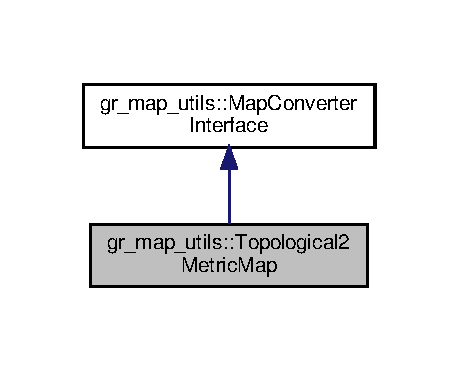
\includegraphics[width=220pt]{classgr__map__utils_1_1Topological2MetricMap__inherit__graph}
\end{center}
\end{figure}


Collaboration diagram for gr\+\_\+map\+\_\+utils\+:\+:Topological2\+Metric\+Map\+:
\nopagebreak
\begin{figure}[H]
\begin{center}
\leavevmode
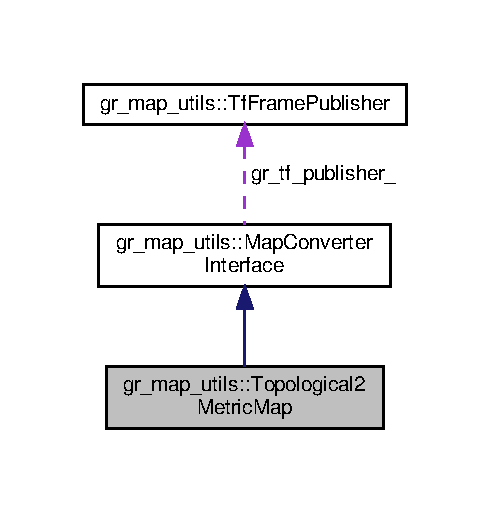
\includegraphics[width=235pt]{classgr__map__utils_1_1Topological2MetricMap__coll__graph}
\end{center}
\end{figure}
\subsection*{Public Member Functions}
\begin{DoxyCompactItemize}
\item 
\mbox{\Hypertarget{classgr__map__utils_1_1Topological2MetricMap_a6d6bf2ea20fb5d385c3bf653abcd62e6}\label{classgr__map__utils_1_1Topological2MetricMap_a6d6bf2ea20fb5d385c3bf653abcd62e6}} 
{\bfseries Topological2\+Metric\+Map} (ros\+::\+Node\+Handle nh, bool initialize\+\_\+tf=true, bool init\+\_\+dyn=true)
\item 
\mbox{\Hypertarget{classgr__map__utils_1_1Topological2MetricMap_accca280444336c009d8edee8881a6c9d}\label{classgr__map__utils_1_1Topological2MetricMap_accca280444336c009d8edee8881a6c9d}} 
virtual bool {\bfseries store\+Map} ()
\item 
\mbox{\Hypertarget{classgr__map__utils_1_1Topological2MetricMap_a0cc94b07abb8f649c93035156615edae}\label{classgr__map__utils_1_1Topological2MetricMap_a0cc94b07abb8f649c93035156615edae}} 
virtual bool {\bfseries get\+Map\+From\+Topic} ()
\item 
\mbox{\Hypertarget{classgr__map__utils_1_1Topological2MetricMap_aa87f17d63a092a0c6b819e25fdbb4923}\label{classgr__map__utils_1_1Topological2MetricMap_aa87f17d63a092a0c6b819e25fdbb4923}} 
virtual bool {\bfseries get\+Map\+From\+Service} ()
\item 
\mbox{\Hypertarget{classgr__map__utils_1_1Topological2MetricMap_a4ec9577561920cfcca32878f233cbf91}\label{classgr__map__utils_1_1Topological2MetricMap_a4ec9577561920cfcca32878f233cbf91}} 
virtual bool {\bfseries get\+Map\+From\+Database} ()
\item 
\mbox{\Hypertarget{classgr__map__utils_1_1Topological2MetricMap_ab0ae2ad72302af1e5e038dc492c2a47a}\label{classgr__map__utils_1_1Topological2MetricMap_ab0ae2ad72302af1e5e038dc492c2a47a}} 
virtual void {\bfseries transform\+Map} ()
\item 
\mbox{\Hypertarget{classgr__map__utils_1_1Topological2MetricMap_a9de68d38f7b4600fc2aecda021888a1b}\label{classgr__map__utils_1_1Topological2MetricMap_a9de68d38f7b4600fc2aecda021888a1b}} 
virtual void {\bfseries publish\+Maps} ()
\item 
\mbox{\Hypertarget{classgr__map__utils_1_1Topological2MetricMap_aae3af8577fb284c46977d1a261613753}\label{classgr__map__utils_1_1Topological2MetricMap_aae3af8577fb284c46977d1a261613753}} 
bool {\bfseries update\+Map} (Update\+Map\+::\+Request \&req, Update\+Map\+::\+Response \&resp)
\item 
\mbox{\Hypertarget{classgr__map__utils_1_1Topological2MetricMap_abc85730ec953ab15735062d8a211bbc2}\label{classgr__map__utils_1_1Topological2MetricMap_abc85730ec953ab15735062d8a211bbc2}} 
void {\bfseries timer\+\_\+cb} (const ros\+::\+Timer\+Event \&event)
\item 
\mbox{\Hypertarget{classgr__map__utils_1_1Topological2MetricMap_a69c5591684631c33e7fe3e1df58c6d03}\label{classgr__map__utils_1_1Topological2MetricMap_a69c5591684631c33e7fe3e1df58c6d03}} 
void {\bfseries dyn\+\_\+reconfigure\+CB} (Topological\+Map\+Converter\+Config \&config, uint32\+\_\+t level)
\end{DoxyCompactItemize}
\subsection*{Additional Inherited Members}


\subsection{Detailed Description}


Definition at line 36 of file topological\+\_\+to\+\_\+metric\+\_\+converter.\+h.



The documentation for this class was generated from the following files\+:\begin{DoxyCompactItemize}
\item 
/home/jose/ros\+\_\+ws/src/gr\+\_\+navigation/gr\+\_\+map\+\_\+tools/gr\+\_\+map\+\_\+utils/include/gr\+\_\+map\+\_\+utils/topological\+\_\+to\+\_\+metric\+\_\+converter.\+h\item 
/home/jose/ros\+\_\+ws/src/gr\+\_\+navigation/gr\+\_\+map\+\_\+tools/gr\+\_\+map\+\_\+utils/src/topological\+\_\+to\+\_\+metric\+\_\+converter.\+cpp\end{DoxyCompactItemize}

\hypertarget{classgr__topological__navigation_1_1states_1_1topological__planner_1_1TopologicalPlanner}{}\section{gr\+\_\+topological\+\_\+navigation.\+states.\+topological\+\_\+planner.\+Topological\+Planner Class Reference}
\label{classgr__topological__navigation_1_1states_1_1topological__planner_1_1TopologicalPlanner}\index{gr\+\_\+topological\+\_\+navigation.\+states.\+topological\+\_\+planner.\+Topological\+Planner@{gr\+\_\+topological\+\_\+navigation.\+states.\+topological\+\_\+planner.\+Topological\+Planner}}


Inheritance diagram for gr\+\_\+topological\+\_\+navigation.\+states.\+topological\+\_\+planner.\+Topological\+Planner\+:
\nopagebreak
\begin{figure}[H]
\begin{center}
\leavevmode
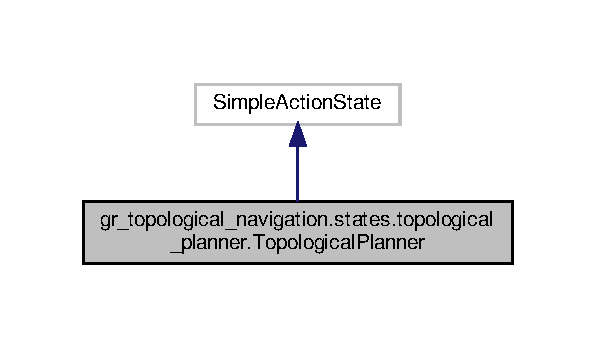
\includegraphics[width=286pt]{classgr__topological__navigation_1_1states_1_1topological__planner_1_1TopologicalPlanner__inherit__graph}
\end{center}
\end{figure}


Collaboration diagram for gr\+\_\+topological\+\_\+navigation.\+states.\+topological\+\_\+planner.\+Topological\+Planner\+:
\nopagebreak
\begin{figure}[H]
\begin{center}
\leavevmode
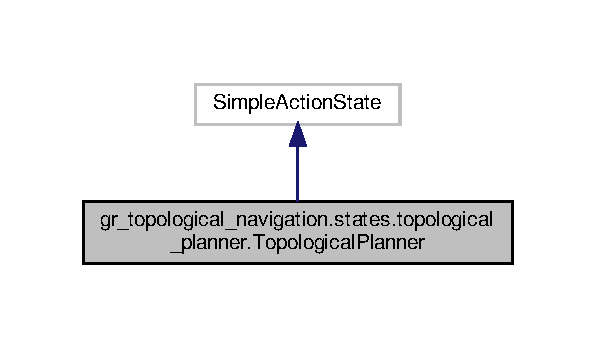
\includegraphics[width=286pt]{classgr__topological__navigation_1_1states_1_1topological__planner_1_1TopologicalPlanner__coll__graph}
\end{center}
\end{figure}
\subsection*{Public Member Functions}
\begin{DoxyCompactItemize}
\item 
\mbox{\Hypertarget{classgr__topological__navigation_1_1states_1_1topological__planner_1_1TopologicalPlanner_a15c9719a888829cc1a0ebb6bd4001e10}\label{classgr__topological__navigation_1_1states_1_1topological__planner_1_1TopologicalPlanner_a15c9719a888829cc1a0ebb6bd4001e10}} 
def {\bfseries \+\_\+\+\_\+init\+\_\+\+\_\+} (self, gui=False, pointset=\char`\"{}hello\+\_\+world\char`\"{}, nav\+\_\+action=\char`\"{}sbpl\+\_\+action\char`\"{})
\item 
\mbox{\Hypertarget{classgr__topological__navigation_1_1states_1_1topological__planner_1_1TopologicalPlanner_a9a418307dc39e24a94dc02ef904fdc21}\label{classgr__topological__navigation_1_1states_1_1topological__planner_1_1TopologicalPlanner_a9a418307dc39e24a94dc02ef904fdc21}} 
def {\bfseries current\+\_\+node\+\_\+callback} (self, node)
\item 
\mbox{\Hypertarget{classgr__topological__navigation_1_1states_1_1topological__planner_1_1TopologicalPlanner_a518b45bcc3e5df8c55aa091942dae1f9}\label{classgr__topological__navigation_1_1states_1_1topological__planner_1_1TopologicalPlanner_a518b45bcc3e5df8c55aa091942dae1f9}} 
def {\bfseries reset\+\_\+graph} (self, amap)
\item 
\mbox{\Hypertarget{classgr__topological__navigation_1_1states_1_1topological__planner_1_1TopologicalPlanner_afa57ae46f7ab4f0c34022a0c4bcc14b4}\label{classgr__topological__navigation_1_1states_1_1topological__planner_1_1TopologicalPlanner_afa57ae46f7ab4f0c34022a0c4bcc14b4}} 
def {\bfseries get\+\_\+map} (self)
\item 
\mbox{\Hypertarget{classgr__topological__navigation_1_1states_1_1topological__planner_1_1TopologicalPlanner_a9fdc701da6d3e24e7133d67a8a27946f}\label{classgr__topological__navigation_1_1states_1_1topological__planner_1_1TopologicalPlanner_a9fdc701da6d3e24e7133d67a8a27946f}} 
def {\bfseries current\+\_\+edge\+\_\+callback} (self, edge\+\_\+raw)
\item 
\mbox{\Hypertarget{classgr__topological__navigation_1_1states_1_1topological__planner_1_1TopologicalPlanner_aca9224c56e49a64b91e66392b92758f3}\label{classgr__topological__navigation_1_1states_1_1topological__planner_1_1TopologicalPlanner_aca9224c56e49a64b91e66392b92758f3}} 
def {\bfseries reset} (self)
\item 
\mbox{\Hypertarget{classgr__topological__navigation_1_1states_1_1topological__planner_1_1TopologicalPlanner_a562b72280078e85979263de577380356}\label{classgr__topological__navigation_1_1states_1_1topological__planner_1_1TopologicalPlanner_a562b72280078e85979263de577380356}} 
def {\bfseries calculate\+\_\+weight} (self, a, b)
\item 
\mbox{\Hypertarget{classgr__topological__navigation_1_1states_1_1topological__planner_1_1TopologicalPlanner_aab09f830998a9c394f6dbf8a2f218837}\label{classgr__topological__navigation_1_1states_1_1topological__planner_1_1TopologicalPlanner_aab09f830998a9c394f6dbf8a2f218837}} 
def {\bfseries create\+\_\+graph} (self, amap)
\item 
\mbox{\Hypertarget{classgr__topological__navigation_1_1states_1_1topological__planner_1_1TopologicalPlanner_a2b2f245bffd94849cca5ee923c9a45fa}\label{classgr__topological__navigation_1_1states_1_1topological__planner_1_1TopologicalPlanner_a2b2f245bffd94849cca5ee923c9a45fa}} 
def {\bfseries generate\+\_\+full\+\_\+coverage\+\_\+plan} (self)
\item 
\mbox{\Hypertarget{classgr__topological__navigation_1_1states_1_1topological__planner_1_1TopologicalPlanner_aa177e70422db2dc1ac8f4c78f3164e03}\label{classgr__topological__navigation_1_1states_1_1topological__planner_1_1TopologicalPlanner_aa177e70422db2dc1ac8f4c78f3164e03}} 
def {\bfseries go\+\_\+to\+\_\+source} (self)
\item 
\mbox{\Hypertarget{classgr__topological__navigation_1_1states_1_1topological__planner_1_1TopologicalPlanner_a0ab5df866803c0730ce9ced9a2da670a}\label{classgr__topological__navigation_1_1states_1_1topological__planner_1_1TopologicalPlanner_a0ab5df866803c0730ce9ced9a2da670a}} 
def {\bfseries get\+\_\+next\+\_\+transition} (self)
\item 
\mbox{\Hypertarget{classgr__topological__navigation_1_1states_1_1topological__planner_1_1TopologicalPlanner_abebef25b3c3a3bfa87fb16a8a01adf5b}\label{classgr__topological__navigation_1_1states_1_1topological__planner_1_1TopologicalPlanner_abebef25b3c3a3bfa87fb16a8a01adf5b}} 
def {\bfseries get\+\_\+orientation} (self, edge)
\item 
\mbox{\Hypertarget{classgr__topological__navigation_1_1states_1_1topological__planner_1_1TopologicalPlanner_a74048f7a02e048e1e9d1356bbe33b5c6}\label{classgr__topological__navigation_1_1states_1_1topological__planner_1_1TopologicalPlanner_a74048f7a02e048e1e9d1356bbe33b5c6}} 
def {\bfseries goal\+\_\+cb} (self, userdata, goal)
\item 
\mbox{\Hypertarget{classgr__topological__navigation_1_1states_1_1topological__planner_1_1TopologicalPlanner_ab449bf1b9cbe9892c600df132d91be1b}\label{classgr__topological__navigation_1_1states_1_1topological__planner_1_1TopologicalPlanner_ab449bf1b9cbe9892c600df132d91be1b}} 
def {\bfseries result\+\_\+cb} (self, userdata, status, results)
\item 
\mbox{\Hypertarget{classgr__topological__navigation_1_1states_1_1topological__planner_1_1TopologicalPlanner_aceac8aeb95962a4620aaebfd950c5dc6}\label{classgr__topological__navigation_1_1states_1_1topological__planner_1_1TopologicalPlanner_aceac8aeb95962a4620aaebfd950c5dc6}} 
def {\bfseries show\+\_\+statistics} (self)
\end{DoxyCompactItemize}
\subsection*{Data Fields}
\begin{DoxyCompactItemize}
\item 
\mbox{\Hypertarget{classgr__topological__navigation_1_1states_1_1topological__planner_1_1TopologicalPlanner_a8d2420f7f708d02174c991cc1c79db09}\label{classgr__topological__navigation_1_1states_1_1topological__planner_1_1TopologicalPlanner_a8d2420f7f708d02174c991cc1c79db09}} 
{\bfseries msg\+\_\+store}
\item 
\mbox{\Hypertarget{classgr__topological__navigation_1_1states_1_1topological__planner_1_1TopologicalPlanner_a4531675f025eeff8b640059a9b1d2745}\label{classgr__topological__navigation_1_1states_1_1topological__planner_1_1TopologicalPlanner_a4531675f025eeff8b640059a9b1d2745}} 
{\bfseries current\+\_\+node}
\item 
\mbox{\Hypertarget{classgr__topological__navigation_1_1states_1_1topological__planner_1_1TopologicalPlanner_aa5eaeb315401f1318dfbd6b3cfe9df44}\label{classgr__topological__navigation_1_1states_1_1topological__planner_1_1TopologicalPlanner_aa5eaeb315401f1318dfbd6b3cfe9df44}} 
{\bfseries gui}
\item 
\mbox{\Hypertarget{classgr__topological__navigation_1_1states_1_1topological__planner_1_1TopologicalPlanner_adff7724371a2867d45f76bfc89bd3fd7}\label{classgr__topological__navigation_1_1states_1_1topological__planner_1_1TopologicalPlanner_adff7724371a2867d45f76bfc89bd3fd7}} 
{\bfseries pointset}
\item 
\mbox{\Hypertarget{classgr__topological__navigation_1_1states_1_1topological__planner_1_1TopologicalPlanner_a1e89775ae6585618d3453d6257edfb68}\label{classgr__topological__navigation_1_1states_1_1topological__planner_1_1TopologicalPlanner_a1e89775ae6585618d3453d6257edfb68}} 
{\bfseries topological\+\_\+plan}
\item 
\mbox{\Hypertarget{classgr__topological__navigation_1_1states_1_1topological__planner_1_1TopologicalPlanner_a3f535445117779547c226a1c48954cb1}\label{classgr__topological__navigation_1_1states_1_1topological__planner_1_1TopologicalPlanner_a3f535445117779547c226a1c48954cb1}} 
{\bfseries nodes\+\_\+poses}
\item 
\mbox{\Hypertarget{classgr__topological__navigation_1_1states_1_1topological__planner_1_1TopologicalPlanner_ae31acfe04d3c4f3b819d546566141b51}\label{classgr__topological__navigation_1_1states_1_1topological__planner_1_1TopologicalPlanner_ae31acfe04d3c4f3b819d546566141b51}} 
{\bfseries is\+\_\+task\+\_\+initialized}
\item 
\mbox{\Hypertarget{classgr__topological__navigation_1_1states_1_1topological__planner_1_1TopologicalPlanner_abb34f0a796fd150a875f920f41c166be}\label{classgr__topological__navigation_1_1states_1_1topological__planner_1_1TopologicalPlanner_abb34f0a796fd150a875f920f41c166be}} 
{\bfseries visited\+\_\+edges}
\item 
\mbox{\Hypertarget{classgr__topological__navigation_1_1states_1_1topological__planner_1_1TopologicalPlanner_a98ec472a7a81b152c51a8ca530fe41cd}\label{classgr__topological__navigation_1_1states_1_1topological__planner_1_1TopologicalPlanner_a98ec472a7a81b152c51a8ca530fe41cd}} 
{\bfseries networkx\+\_\+graph}
\end{DoxyCompactItemize}


\subsection{Detailed Description}


Definition at line 22 of file topological\+\_\+planner.\+py.



The documentation for this class was generated from the following file\+:\begin{DoxyCompactItemize}
\item 
/home/jose/ros\+\_\+ws/src/gr\+\_\+navigation/gr\+\_\+navigation\+\_\+managers/gr\+\_\+topological\+\_\+navigation/src/gr\+\_\+topological\+\_\+navigation/states/topological\+\_\+planner.\+py\end{DoxyCompactItemize}

%--- End generated contents ---

% Index
\backmatter
\newpage
\phantomsection
\clearemptydoublepage
\addcontentsline{toc}{chapter}{Index}
\printindex

\end{document}
